\documentclass[a4paper,11pt]{article}

\usepackage[toc,page]{appendix}
\usepackage{listings}
\usepackage{appendix}
\usepackage[utf8]{inputenc}
\usepackage[T1]{fontenc}
\usepackage[a4paper,left=2cm,right=2cm,top=2cm,bottom=2cm]{geometry}
\usepackage[english,french]{babel}
\usepackage{fullpage}
\usepackage{setspace}
\usepackage[pdftex]{graphicx}
\usepackage{wrapfig}
\usepackage{soul}
\usepackage{pdflscape}
\usepackage{amsmath}
%\usepackage{ucs}
\usepackage{fancyhdr}
\usepackage{intcalc}
\usepackage{mathastext}
\usepackage{amsthm}
\usepackage{datetime}
\usepackage{xspace}
\usepackage{hyperref}
\usepackage[all]{hypcap}
\usepackage{tikz}
\usepackage{enumerate}
\usepackage{color}
\usepackage{setspace}
\usepackage{here}
\usepackage{titlesec}
\usepackage{pdfpages}
\usepackage{caption}
\usepackage{tcolorbox}
\usepackage{scrextend,rotating}
\usepackage[backend = biber, style = nature, sorting = none]{biblatex}
\addbibresource{biblio.bib}
\usepackage{eurosym}
\usepackage{comment}
\usepackage{framed}
\usepackage{gensymb}
\usepackage{array}
\usepackage{multirow}
\usepackage{diagbox}

\renewcommand{\appendixpagename}{\Large{Annexes}}
\renewcommand{\appendixtocname}{Annexes}
 

\hypersetup{colorlinks,citecolor=black,filecolor=black,linkcolor=black,urlcolor=black}

\linespread{1.5}
\AddThinSpaceBeforeFootnotes 
\FrenchFootnotes
\setlength{\parindent}{1cm}
\setlength{\parskip}{1ex plus 0.5ex minus 0.2ex}
\newcommand{\hsp}{\hspace{20pt}}
\newcommand{\HRule}{\rule{\linewidth}{0.5mm}}

\begin{document}

\begin{titlepage}
    \linespread{1}
    	\begin{center}
            \begin{framed}
              \parbox[c][13mm]{215pt}{
                \scriptsize\sf           École polytechnique de Bruxelles\\
                \scriptsize\sf           Bachelier en sciences de l'ingénieur, orientation ingénieur civil\\
                \scriptsize\sf           Deuxième année\\
                \scriptsize\sf           TRAN-H201 - Projet multidisciplinaire II
                }
                \hfill
              \parbox[c][13mm]{178.52396pt}{
\includegraphics[height=13mm]{logo_EPB.jpg}}
            \end{framed}\\[1cm]
            
	%	
\includegraphics[height = 15mm]{logo_EPB.jpg}~\\[1.5cm]
		
		\textsc{\Large Université libre de Bruxelles}\\[1.5cm]
		
		\hrule
		%\begin{framed}
		\begin{framed}{\Large\bfseries \ Projet d'électromécanique :\\ \LARGE Conception et réalisation d'un robot magasinier\\ \Large Rapport de fin de parcours}
		\end{framed}
		%\end{framed}
		\hrule
		
		\vspace{12mm}
		
		\begin{minipage}[t]{0.6\textwidth}
			\begin{center} \large
			\emph{Tuteur :}            \\
			\vspace{2mm}
			Ir. Max \textsc{Thulliez}
			\end{center}
		\end{minipage}
		
		\hsp
		
		\begin{minipage}[t]{0.6\textwidth}
			\begin{center} \large
				\emph{Auteurs :}            \\
				\vspace{2mm}
                Loïc \bsc{Dewitte}          \\
                Maxime \bsc{Renard}         \\
                Théo \bsc{Saclier}          \\
                Firas \bsc{Samaan}          \\
                Tristan \bsc{Smeesters}     \\
                Julien \bsc{van Delft}
			\end{center}
		\end{minipage}
			
		\vfill
			
		
\includegraphics[height = 25mm]{sceau.jpg} \\
		\vspace{5mm}
		{\large Belgique \\2019}
	\end{center}
\end{titlepage}
\cleardoublepage

\pagenumbering{roman}
\tableofcontents
%\clearpage
%\pagenumbering{Roman}

%\noindent Nombre de mots du rapport :  \\
%Nombre de caractères de l'abstract :  (espaces non compris)

%\section*{Abstract}
%\section*{But}

\cleardoublepage
\pagenumbering{arabic}

\section{Introduction}

Dans le cadre de leur deuxième année de bachelier à l'École polytechnique de Bruxelles, les étudiants ont été rassemblés par groupe de 6 ou 7 membres afin de réaliser un projet dans la filière de leur choix. Dans la section électromécanique choisie par notre groupe, il s'agit de mettre au point un robot magasinier capable d'effectuer plusieurs tâches définies dans le guide de projet fourni aux étudiants, le tout en moins de deux quadrimestres. Pour ce faire, différents outils sont mis à disposition des groupes de projet: imprimantes 3D, découpeuses lasers ou encore machines CNC (computer numerical control). Les composants nécessaires sont quant à eux à déterminer et à se procurer par le groupe, dont certains par l'intermédiaire de l'École. Ainsi, chaque groupe possède un certain degré de liberté quant à la réalisation et au développement d'un design adapté à la stratégie mise en place pour accomplir la mission imposée.

Le présent rapport détaille en premier lieu le but du projet, ses objectifs ainsi que le cahier des charges qui en a été tiré. Ensuite, la stratégie d'exécution de l'action demandée au robot est déterminée, menant à la présentation du design du robot, de ses composants et de la construction de celui-ci. Le fonctionnement global du robot est alors présenté, suivi par le développement de l'odométrie mise en place ainsi que de la régulation. S'en suit un mot sur les simulations employées afin de tester le fonctionnement prévu du robot, ainsi que sur les tests en temps réel. Finalement, les résultats de l'ensemble du projet sont présentés, et les optimisations futures possibles sont discutées. La gestion de projet adoptée et employée tout du long clôture le rapport écrit. Les codes se trouvent en annexe.

\clearpage
\section{\label{sec: desc}Description du projet}

\subsection{Objectif}

Le robot magasinier doit être capable de déplacer des flacons de diamètre différent depuis leur emplacement jusqu'à une zone de dépôt. Ainsi, sur un terrain représentant la configuration d'une usine (voir figure \ref{fig:schéma} ci-dessous), se trouvent trois zones : deux zones de dépôt et une zone de production. Ce terrain possède une largeur et une longueur respectives d'approximativement 1,5m et de 2,5m. Les emplacements sur lesquels seront disposés des flacons se situent sur un parcours préétabli, marqué par de l'autocollant noir. Ce parcours mesure approximativement 14m. Six flacons sont arbitrairement disposés sur six des douze emplacements possibles. Il existe trois sortes de flacons, de diamètres différents; il y aura donc deux flacons de chaque sorte. Le robot doit ramener les petits et grands flacons respectivement dans les zones pour petits et grands flacons. Ceux de taille moyenne doivent rester en place.

\begin{center}
    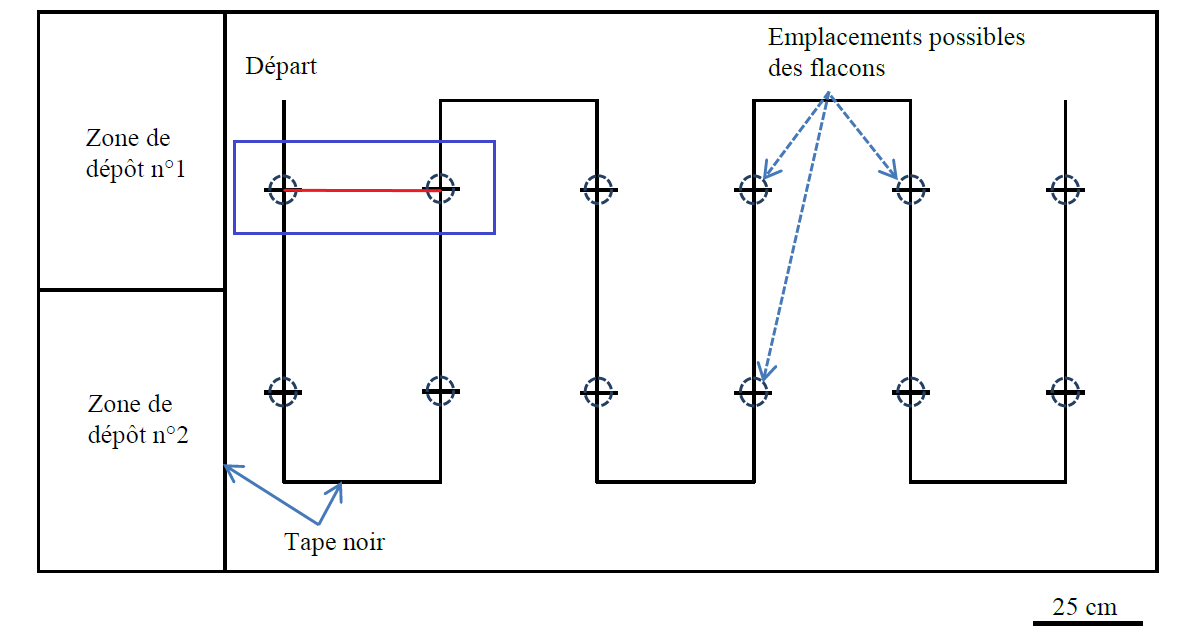
\includegraphics[height=80mm]{schema_circuit.png}
    \captionof{figure}{\label{fig:schéma}Schéma du terrain \cite{guide}}
\end{center}    

Il est demandé aux étudiants de s'occuper de la conception, des plans, de la sélection des composants, de la construction, de la programmation et des tests du robot. Des équipements (Fablab, laboratoires) et formations sont mis à disposition par l'École, complétés par l'achat de matériel par le groupe et par les tuteurs du projet.

\subsection{Cahier des charges}

Un cahier des charges a pu être dégagé des objectifs et consignes fixées par le guide \cite{guide}, imposant dès lors certaines contraintes et limitations.

Ainsi, le budget maximal est de 100 euros. Il doit inclure le coût des composants commandés (par les superviseurs ou par le groupe, à l'exception de la batterie), mais n'intègre pas le matériel récupéré dans le local projet, au Polystock ou autre, ni les frais d'utilisation des équipements mis à disposition (imprimantes 3D, découpeuses, etc.).

Considérant la géométrie du terrain et afin que le robot puisse s'y déplacer librement, la distance limitante sur le terrain est ressortie comme étant la plus petite distance entre deux tubes de diamètre large. Celle-ci se trouve indiquée sur la figure \ref{fig:schéma} par un trait rouge dans le rectangle bleu. Cette distance est théoriquement de 318mm, et une large distance de sécurité de 47,5mm y est appliquée de chaque côté. En effet, la réalisation de ce genre de robot est une première pour le groupe, et un intervalle de sécurité de 30\% a été jugé raisonnable. La largeur maximale du robot en résultant est de 223mm. La longueur maximale a été elle déterminée comme étant la distance entre deux tubes larges calculée dans le couloir central du terrain. Celle-ci est de 400mm, sécurisée selon le même critère à 280mm.

Six tubes en PVC, d'une hauteur de 60mm et d'un diamètre de 32, 40 ou 50mm (deux de chaque diamètre) représentent les flacons à récupérer. Le robot doit donc être capable de les identifier et les différentier, afin d'attraper les petits et larges tubes. Ceux de diamètre intermédiaire ne doivent pas être pris. Les petits et larges tubes doivent ensuite être transportés jusqu'à une zone où ils seront rangés dans la sous-zone qui est dédiée à leur diamètre (les tubes de 32mm de diamètre dans la zone pour petits tubes et ceux de 50mm dans la zone pour larges tubes).

Le temps maximal pour l'accomplissement de la tâche du robot est de 5 minutes.

\vspace{3mm}
\begin{center}
\begin{tabular}[h!]{l p{11.1cm}}
    \multicolumn{2}{c}{\textbf{Cahier des charges}}
    \vspace{4mm}
    \\
    \hline
    Budget & Le budget ne peut dépasser \EUR{100} en commandes (sauf batterie).\\
    \hline
    Dimensionnement & La largeur maximale du robot est de 223mm.\\ & La longueur maximale du robot est de 280mm.\\
    \hline
    Identifier des tubes & Des tubes de 60mm de hauteur et d'un diamètre de 32mm, 40mm et 50mm doivent être identifiés.\\ \hline
    Saisie des tubes & Les tubes de 32mm et 50mm de diamètre doivent être saisis. \\
    & Les tubes d'un diamètre de 40mm doivent être laissés sur place. \\ \hline
    Transport des tubes & Les tubes saisis doivent être transportés jusqu'à leur zone de dépôt. \\ \hline
    Dépôt des tubes & Les tubes transportés doivent être déposés dans la zone allouée à leur diamètre. \\ \hline
    Durée & La tâche doit être entièrement complétée en moins de 5 minutes.\\ \hline
    \label{cdc}
\vspace{-2mm}
\end{tabular}
\captionof{table}{Cahier des charges}
\end{center}
\clearpage

\section{Stratégie d'exécution}

Plusieurs stratégies de fonctionnement du robot (déplacement, préhension, différentiation des tubes, etc.) ont été confrontées avant d'arriver au choix final. Ce choix plus approprié a ensuite défini le design du robot.

Dans cette section, différents points seront abordés dans l'ordre suivant : stratégie de déplacement, choix de conserver ou non les tubes, puis stratégies de prise des tubes et de leur détection préalable.

\subsection{\label{subsec:choix}Déplacement}

Une première possibilité de déplacement du robot consiste en le suivi du tracé d'adhésif noir. Ainsi, il se repérerait sur le terrain grâce au tracé (à l'aide de capteurs de bord, par exemple) et devrait effectuer les manoeuvres liées aux tubes en restant sur le tape, voire en le quittant et y retournant par après. Ces manoeuvres seraient plus délicates pour les tubes moyens : il faudrait les contourner, les lever pour les replacer, ou passer au dessus. Il serait également nécessaire de stocker les tubes à récupérer ou d'effectuer des aller-retours chronophages - il faudrait à  chaque fois suivre une partie du tracé dans les deux sens. L'avantage principal était la non nécessité d'une odométrie pour repérer le robot.

\begin{figure}[H]
    \centering
    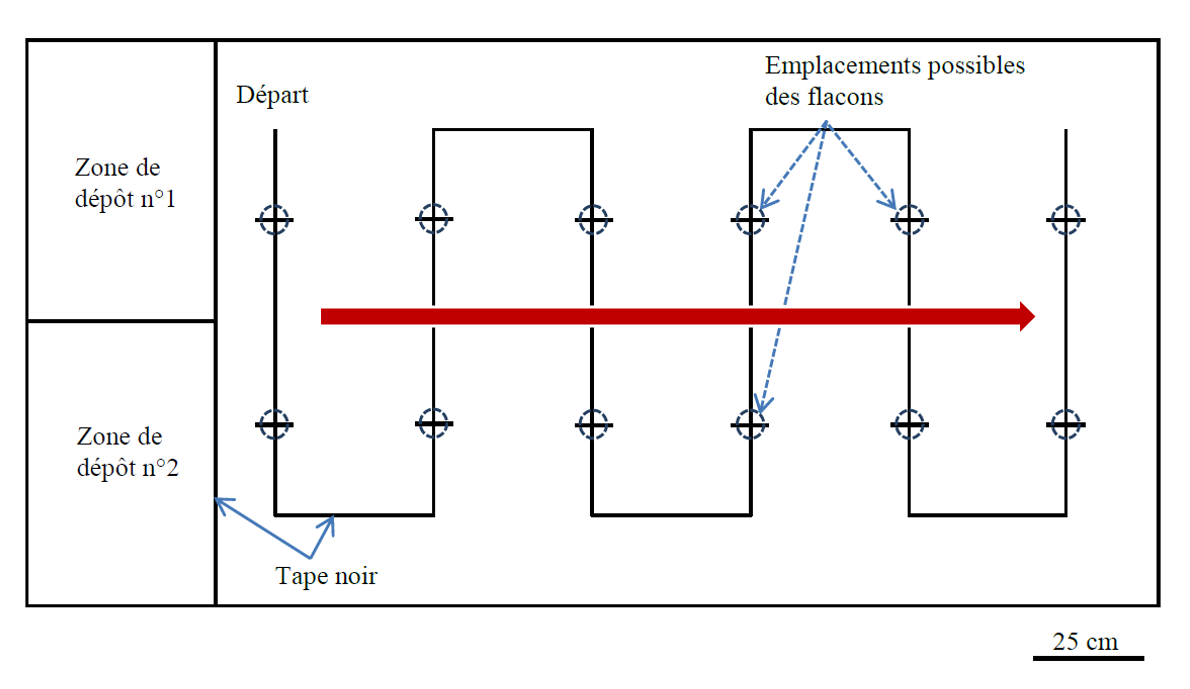
\includegraphics[scale = 0.4]{sens_parcours.PNG}
    \caption{Traversée du parcours}\label{parcours}
\end{figure}
\newpage

Une deuxième possibilité impliquait la traversée du parcours en son centre, c'est à dire horizontalement en traversant les lignes verticales sur la figure \ref{parcours}. Le robot ne suivrait donc pas l'adhésif, permettant gain de temps considérable. Une odométrie (module calculant la position et l'orientation du robot) semblait par contre nécessaire.

La table \ref{compdep} reprend les différents avantages des deux possibilités et les compare.

\vspace{3mm}
\begin{center}
    \begin{tabular}{c | c | c}
    \backslashbox{Critères}{Stratégie} & Suivi de l'adhésif & Traversée centrale \\ \hline
	Complexité des manoeuvres & + (tubes moyens) & - \\ \hline
	\multirow{2}{*}{Repérage} & \multirow{2}{*}{Grâce au tracé et à des capteurs de bord} & Odométrie \\
	& & Rien\\ \hline
	Temps de parcours & Long & Court\\ \hline
	\multirow{2}{*}{Autre} & Implique stockage des tubes moyens, & \multirow{2}{*}{/} \\
	& remise en place ou contournement & \\
\end{tabular}
\vspace{5mm}
\captionof{table}{\label{compdep}Comparatif des possibilités de déplacement}
\end{center}

La stratégie de déplacement retenue est la seconde. Une odométrie a donc été développée et est expliquée au point \ref{sec:odo}.

\subsection{Conservation, transport unitaire}

Deux possibilités sont envisageables quant à la stratégie de prise des tubes : les stocker sur ou sous le robot, ou les ramener un à un.

La conservation des tubes nécessitait une zone aménagée à cet effet sur le robot, augmentant ses dimensions. Cela réduirait soit sa maniabilité en agrandissant la taille de la base du robot, soit sa stabilité en l'agrandissant en hauteur. La complexité des manoeuvres de prise de tubes en serait également augmentée. Toutefois, le gain de temps serait considérable.

En transportant un tube à la fois, l'action de prise serait plus basique, et les dimensions pourraient être plus réduites. Le robot pourrait être aisément adapté à une situation similaire où le nombre de tubes changerait. Sa robustesse en cas de changement de configuration en serait ainsi accrue, tout comme sa versatilité.
\newpage

La table \ref{compcons} reprend les différents avantages des deux possibilité et les compare.

\vspace{3mm}
\begin{center}
    \begin{tabular}{c | c | c}
    \backslashbox{Critères}{Stratégie} & Conservation & Transport unitaire \\ \hline
	\multirow{2}{*}{Dimensionnement} & Plus grande base & \multirow{2}{*}{Compacité}\\ 
	& Plus haut & \\ \hline
	Maniabilité & - (base) & ++ \\ \hline
	Stabilité & - (hauteur) & + \\ \hline
	Complexité des manoeuvres de prise & + & - - \\ \hline
	Versatilité & / & ++ \\ \hline
	Temps d'exécution & - - & + \\
\end{tabular}
\vspace{5mm}
\captionof{table}{\label{compcons}Comparatif des possibilités de conservation des tubes}
\end{center}

Il a été décidé de transporter un tube à la fois, sans en conserver plusieurs simultanément sur le robot.

\subsection{Prise des tubes}

Le transport des tubes en les poussant sur le sol a été rejeté de prime abord, la qualité de la surface pouvant être très approximative. La surface pourrait mener à trop de frottement pour que la pousse des tubes se fasse correctement, ou être trop peu lisse pour que ceux-ci ne restent debout. Un système de préhension flexible comme une pince permettrait d'ailleurs également une adaptation à une situation où des tubes de diamètre plus variés seraient employés, alors que la création d'une zone de pousse sur le robot serait plus limitante.

Se proposaient deux pinces : une pince traditionnelle (attrapant les tubes de face), ou une pince attachée à une "grue", venant attraper les tubes par le dessus. La pince traditionnelle est plus simple et sûre, parce que plus basique, répandue et employée. La "grue" amenait une incertitude quant au possible glissement des tubes dans celle-ci lors de la préhension : pouvant potentiellement tomber, vaciller ou se positionner de manière oblique, la "grue" assure un transport et une pose des tubes plus complexe.
\newpage

La table \ref{compprise} reprend les différents avantages de chaque technologie et les compare.

\vspace{3mm}
\begin{center}
    \begin{tabular}{c | c | c | c}
    \multirow{2}{*}{\backslashbox{Critères}{Stratégie}} & \multirow{2}{*}{Pousser les tubes} & \multicolumn{2}{c}{Pince} \\ \cline{3-4}
    & & Traditionnelle & Grue \\ \hline
	Dépendance au terrain & ++ & \multicolumn{2}{c}{- - -} \\ \hline
	Flexibilité & - & \multicolumn{2}{c}{++} \\ \hline
	Simplicité & ++ & + & - - \\ \hline
	Robustesse & Incertaine & ++ & Incertaine \\
\end{tabular}
\vspace{5mm}
\captionof{table}{\label{compprise}Comparatif des possibilités de prise des tubes}
\end{center}

La pince traditionnelle a donc été le système de préhension choisi. Afin que les tubes soient soulevés et ne soient plus en contact avec le sol lors du déplacement du robot, une système élévateur est nécessaire à cette pince.

Une nouvelle fois, deux possibilités : un système élévateur vertical avec crémaillère, et l'emploi d'un moteur rotatif pour incliner et relever la pince.

Le système avec crémaillère est plus complexe, et les frottements dus à la crémaillère risqueraient d'être trop importants. Le développement d'un plus grand nombre de pièces mécanique est également rebutant.

Pour relever la pince avec un moteur rotatif, il faut fixer directement tout le système sur le moteur, à l'aide de pièces mécaniques ou de colle.

La table \ref{compelev} reprend les différents avantages des deux systèmes et les compare.

\vspace{3mm}
\begin{center}
    \begin{tabular}{c | c | c}
    \backslashbox{Critères}{Stratégie} & Crémaillère & Moteur rotatif \\ \hline
	Complexité & ++ & - - \\ \hline
	Frottements & + & Dûs au moteur \\ \hline
	Développement & Plus long et complexe & Simple\\
\end{tabular}
\vspace{5mm}
\captionof{table}{\label{compelev}Comparatif des possibles de systèmes élévateurs}
\end{center}

Le système élévateur retenu est celui du moteur rotatif.

\subsection{\label{detec}Détection}

Trois types de mesures du diamètre des tubes se présentaient : une mesure mécanique exploitant le servomoteur contrôlant la fermeture de la pince, une mesure à distance ou une mesure rapprochée à l'aide de capteurs infrarouges. En plus de la mesure, ces capteurs peuvent aussi donner la distance à laquelle se trouve chaque tube du robot.

La mesure via la pince nécessiterait un capteur de pression supplémentaire ou l'utilisation d'un servomoteur avec feedback. De plus, celle-ci serait hautement inefficace dans le cas d'une fragmentation de l'action du robot en une phase de détection suivie d'une phase de récupération, et obligerait une répétition de l'action de détection et de récupération par tube (en plus des aller-retours). Cette répétition augmente fortement la durée d'exécution.

La mesure à distance permettrait cette fragmentation, qui semble bien plus rapide, mais serait moins précise à cause des capteurs infrarouges nécessaires. En effet, la précision des capteurs est imparfaite et la présence de bruit est à prendre en compte. Par contre, l'utilisation de cette mesure permettrait de mesurer les tubes des deux rangées lors d'un même passage. Des capteurs Sharp GP2D120X à rayons infrarouges \cite{captdist} étaient d'ailleurs disponibles directement à l'École, évitant une commande coûteuse en temps.

La mesure rapprochée avec capteurs offrirait les mêmes possibilités de fragmentation, et sa précision serait plus importante. Cependant, elle nécessiterait un passage auprès de chaque rangée de tubes ou un rapprochement de chaque tube pour mesurer l'ensemble des tubes.

La table \ref{compmes} reprend les différents avantages de chaque technologie et les compare.

%\vspace{3mm}
\begin{center}
    \begin{tabular}{c | c | c | c}
    \backslashbox{Critères}{Mesure} & Au contact & Á distance & Rapprochée \\ \hline
	\multirow{2}{*}{Capteurs nécessaires} & Pression & Infrarouges & \multirow{2}{*}{Infrarouges}\\ 
	& Servomoteur avec feedback & \ & \ \\ \hline
	\multirow{2}{*}{Fragmentation de l'action} & \multirow{2}{*}{- -} & ++ & \multirow{2}{*}{++} \\
	\ & \ & (détection rapide) & \ \\ \hline
	\multirow{2}{*}{Répétition de l'action} & \multirow{2}{*}{++} & \multirow{2}{*}{/} & +\\ 
	& & & ++ \\ \hline
	Précision & ++ & + - & + \\ 
\end{tabular}
\vspace{5mm}
\captionof{table}{\label{compmes}Comparatif des possibles méthodes de mesure des tubes}
\end{center}

La mesure avec capteurs de distance a été privilégiée pour la fragmentation de l'action et la mesure possible de tous les tubes en un passage.

La séquence d'exécution complète reprenant le dépôt du robot, son déplacement, la gestion des tubes, etc. est reprise à la section \ref{fonctionnement} "Fonctionnement global du robot" page \pageref{fonctionnement}.

\clearpage
\section{\label{sec:design}Design du robot et choix des composants}

Le design du robot et le choix de ses différents composants sont ici détaillés. La structure globale du robot sera d'abord abordée avant une discussion plus profonde concernant ses caractéristiques.

\subsection{Châssis}
\begin{figure}[H]
        \centering
        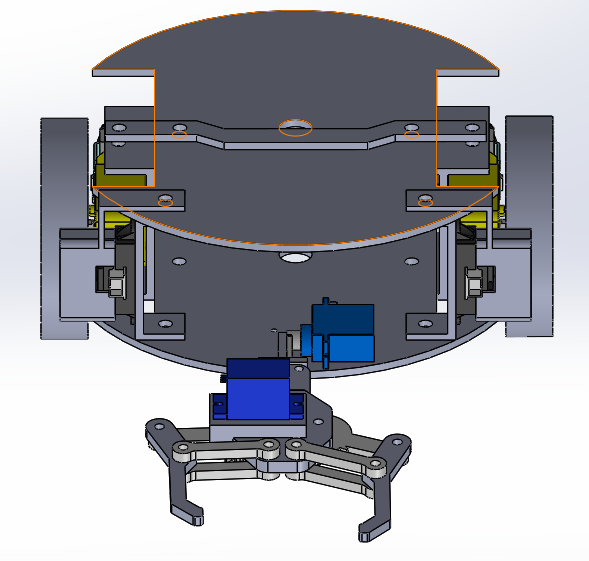
\includegraphics[scale = 0.8]{robot_nu.PNG}
        \captionof{figure}{\label{fig:robot_nu}Avant du châssis sans composantes vu en plongée}
    \hfill
\end{figure}

Le cahier des charges (point \ref{cdc} page \pageref{cdc}) imposait l'utilisation d'un châssis circulaire d'un diamètre d'au plus 223mm. Le châssis est composé de deux étages afin de pouvoir mieux répartir les composants. En privilégiant ainsi la hauteur à la largeur, le robot est plus mobile et moins limité dans ses mouvements. En considérant que la pince dépasse légèrement du véhicule et par mesure de sécurité, le diamètre final a été fixé à 17cm, suffisant pour agencer tous les composants.

\subsection{Roues}

Pour le choix des roues, deux possibilités ont été envisagées : l'utilisation de roues omnidirectionnelles, ou la combinaison de roues motrices avec des roues folles, en l'occurrence des ballcasters.

Les roues omnidirectionnelles (voir figure (\ref{fig:mecanum})) ont suscité une attention pour différentes raisons. Premièrement, celles-ci ont la possibilité de faire se déplacer le robot perpendiculairement au sens traditionnel. Cela aurait permis une grande simplicité dans les déplacements du véhicule, surtout sur un terrain relativement cartésien. Le robot aurait pu évoluer librement en se positionnant juste devant une ligne noire et en se déplaçant parallèlement à celle-ci. Toutefois, deux soucis majeurs se présentent avec ces roues : leur prix élevé (les moins chères sur RobotShop sont à 25\$/pièce \cite{prixrouemeca}), hors budget, et la détermination du modèle dynamique, complexe, afin de concevoir l'odométrie et la régulation. De plus pour qu'un tel modèle puisse être mis en place, 3 roues mécanums sont nécessaires au minimum.

Il aurait été possible de diminuer les coûts en concevant et imprimant en 3D les roues. De nombreux plans 3D sont disponibles gratuitement sur internet. Toutefois, l'incertitude quant au résultat final a fait rejeter cette idée. Le plastique utilisé pour l'impression ne conviendrait peut-être pas et risquerait d'être trop lisse pour que les roues puissent rouler correctement. La précision lors de la conception est également incertaine. Le couple de forces nécessaire pour les mobiliser risquerait également d'être trop important dans le cas de frottements trop faibles sur le terrain.

\begin{figure}[H]
    \begin{minipage}[c]{.46\linewidth}
        \centering
        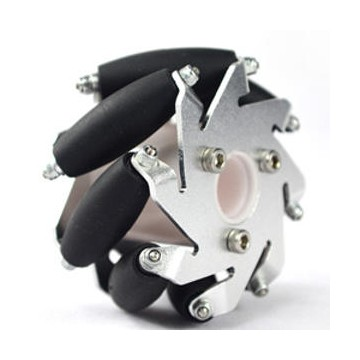
\includegraphics[height = 120]{mecanum.jpg}
        \captionof{figure}{\label{fig:mecanum}Roues omnidirectionnelles \cite{mecanum}}
    \end{minipage}
    \hfill
    \begin{minipage}[c]{.46\linewidth}
        \centering
        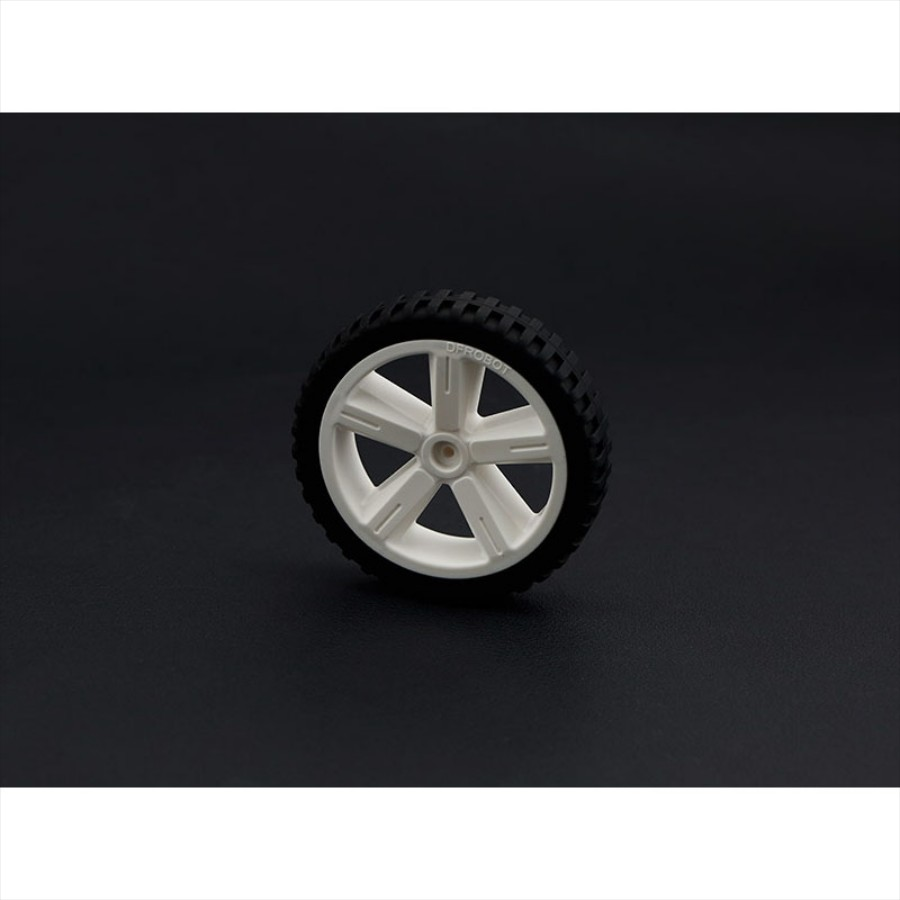
\includegraphics[height = 150]{Roues.jpg}
        \captionof{figure}{\label{fig:Roues}Roue de Silicone de 80mm pour Moteur TT \cite{roues}}
    \end{minipage}
\end{figure}
\newpage

La table \ref{comproues} reprend les différents avantages des modèles de roues et les compare.

\begin{center}
    \begin{tabular}{c | c | c}
    \backslashbox{Critères}{Possibilités} & Roues omnidirectionnelles & Roues motrices \\ \hline
    Prix & Élevé & Tout type de budget \\ \hline
    Complexité de modélisation dynamique & ++ & - - \\ \hline 
    Rapidité du robot & ++ & + \\ \hline
    Maniabilité & ++ & +\\ \hline
    Nombre de roues motorisées minimum & 3 & 2 \\
\end{tabular}
\vspace{5mm}
\captionof{table}{\label{comproues}Comparatif des roues possibles}
\end{center}

Le choix final est constitué de deux roues motrices et de roues libres. Deux roues motrices sont suffisantes pour réaliser toutes les manoeuvres nécessaires. Les roues libres sont des roulettes à bille multidirectionnelles. Elles ont été préférées à de petites roues par souci de fluidité. Elles assurent la bonne stabilité du robot. Les deux roues motrices sont des roues en silicone de 80mm de diamètre \cite{roues} (voir figure \ref{fig:Roues}). Celles-si sont munies d'un moyeu de roue en matériau ABS de bonne qualité.

\subsection{Pince}

Comme annoncé précédemment, le robot attrape les tubes à l'aide d'une pince et ne les conserve pas, devant effectuer des aller-retours pour les déposer. Le choix de la pince s'est porté sur un modèle léger imprimé en 3D. Il s'agit d'un modèle trouvé sur internet \cite{modele_pince} et modifié dans le cadre du projet. Le modèle est simple et s'actionne avec un système d'engrenage. La pince se redresse pour soulever les tubes et les déplacer comme précisé précédemment. Son dimensionnement a été déterminé directement en fonction de la taille des tubes afin que la pince soit capable de saisir les petits mais aussi les grands tubes. De fait, elle possède une ouverture de $6.5cm$ ce qui correspond à la taille des tubes plus $0.75cm$ de sécurité afin de pouvoir prendre et déposer les tubes.

\begin{figure}[H]
    \begin{minipage}[c]{.46\linewidth}
        \centering
        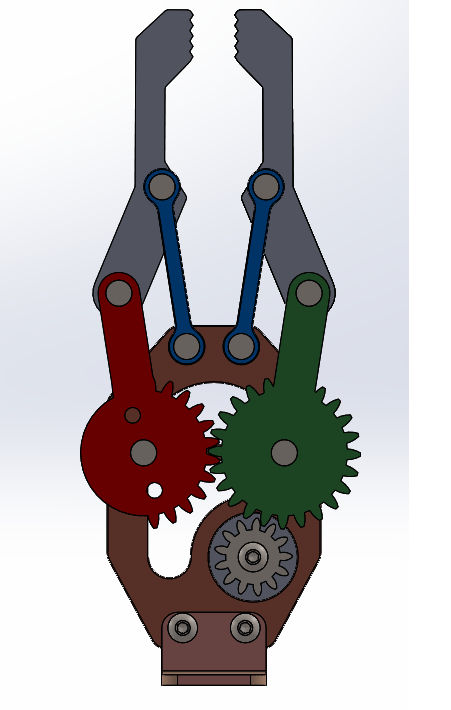
\includegraphics[height = 120]{pince_ferm.png}
        \captionof{figure}{\label{fig:pinceferm}Pince fermée}
    \end{minipage}
    \hfill
    \begin{minipage}[c]{.46\linewidth}
        \centering
        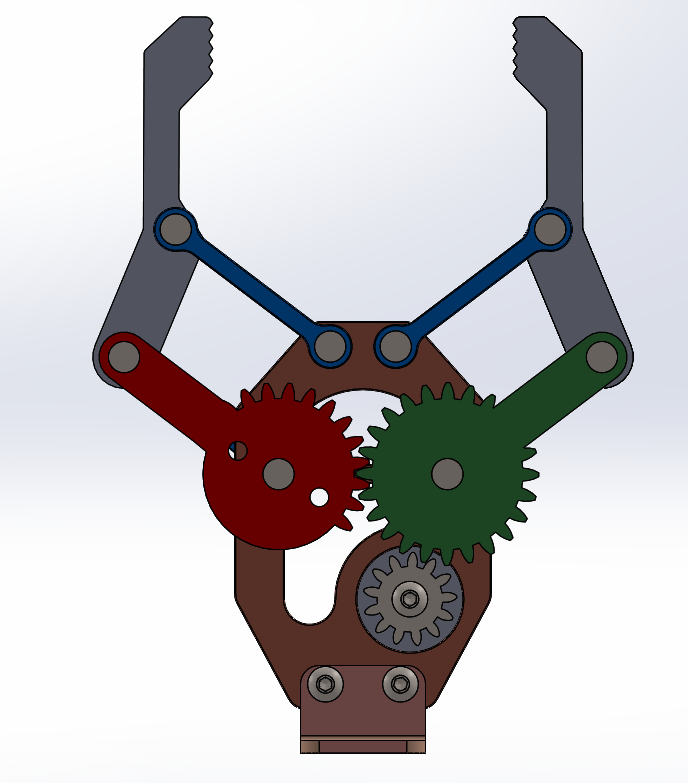
\includegraphics[height = 120]{pince_ouv.png}
        \captionof{figure}{\label{fig:pinceouv}Pince ouverte}
    \end{minipage}
\end{figure}

Les moteurs ainsi que la structure de la pince sont fixés à l'étage du bas. Seuls les bras dépassent afin de ne pas agrandir le diamètre du robot inutilement. La pince est munie de 2 servomoteurs, le premier responsable de sa fermeture et le second dédié au système d'inclinaison.

\subsection{Moteurs}

Plusieurs types de moteurs ont été prévus pour le bon fonctionnement du robot : deux responsables du déplacement et deux pour actionner la pince et son élévation.

Pour le système locomoteur, le choix s'est porté sur deux micro moteurs à encodeur optique de 6V \cite{moteur_encodeur}. Ils peuvent tourner jusqu'à 160 tours/min et leurs encodeurs ont une précision de 1920 tics par tour - plus que suffisante pour l'odométrie et la régulation. Le fournisseur indique également que ces moteurs sont idéaux pour un projet de robotique mobile. Leur prix est raisonnable et entre aisément dans le budget. Le couple de démarrage maximum est de 0,8 kgf.cm et le couple nominal est 0,2 kgf.cm. Ces moteurs sont donc idéals pour notre projet, le couple est suffisant pour réaliser les manoeuvres désirées sans problèmes.

\begin{figure}[H]
    \begin{minipage}[c]{.46\linewidth}
        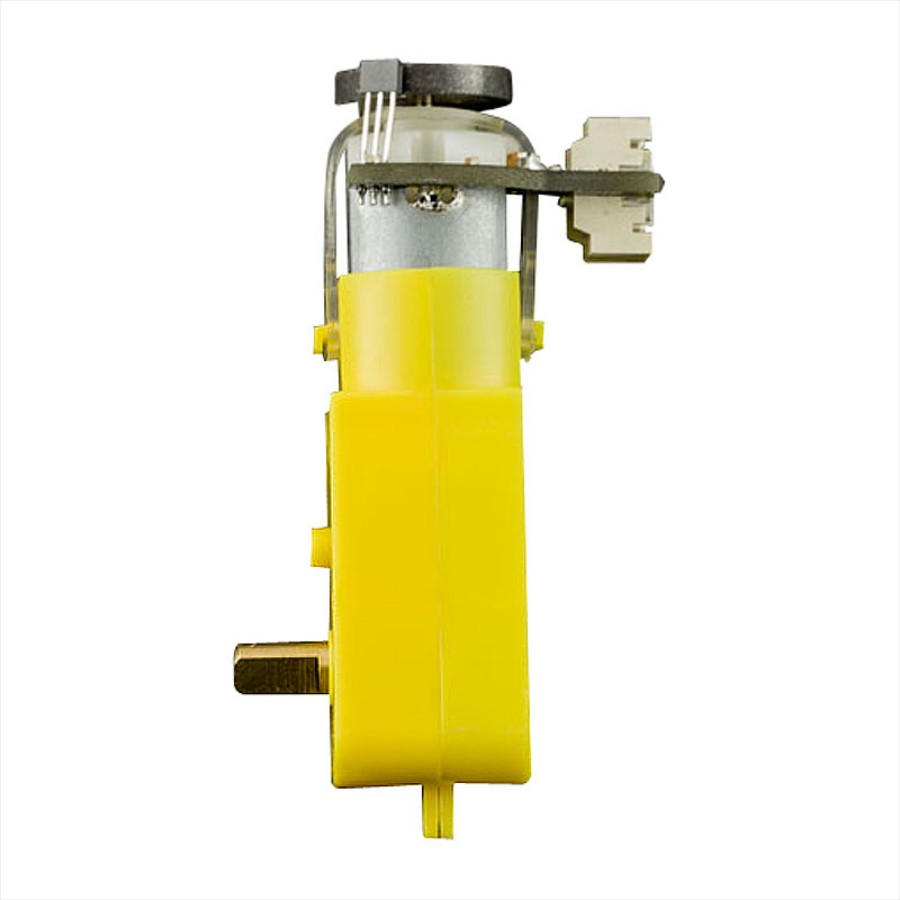
\includegraphics[scale = 0.2]{moteurs_encod.jpg}
    \caption{Micro Moteur DC 6V 160RPM 120:1 avec Encodeur \cite{moteur_encodeur}}
    \label{fig:moteur_encodeur}
    \end{minipage}
    \hfill
    \begin{minipage}[c]{.46\linewidth}
        \centering
    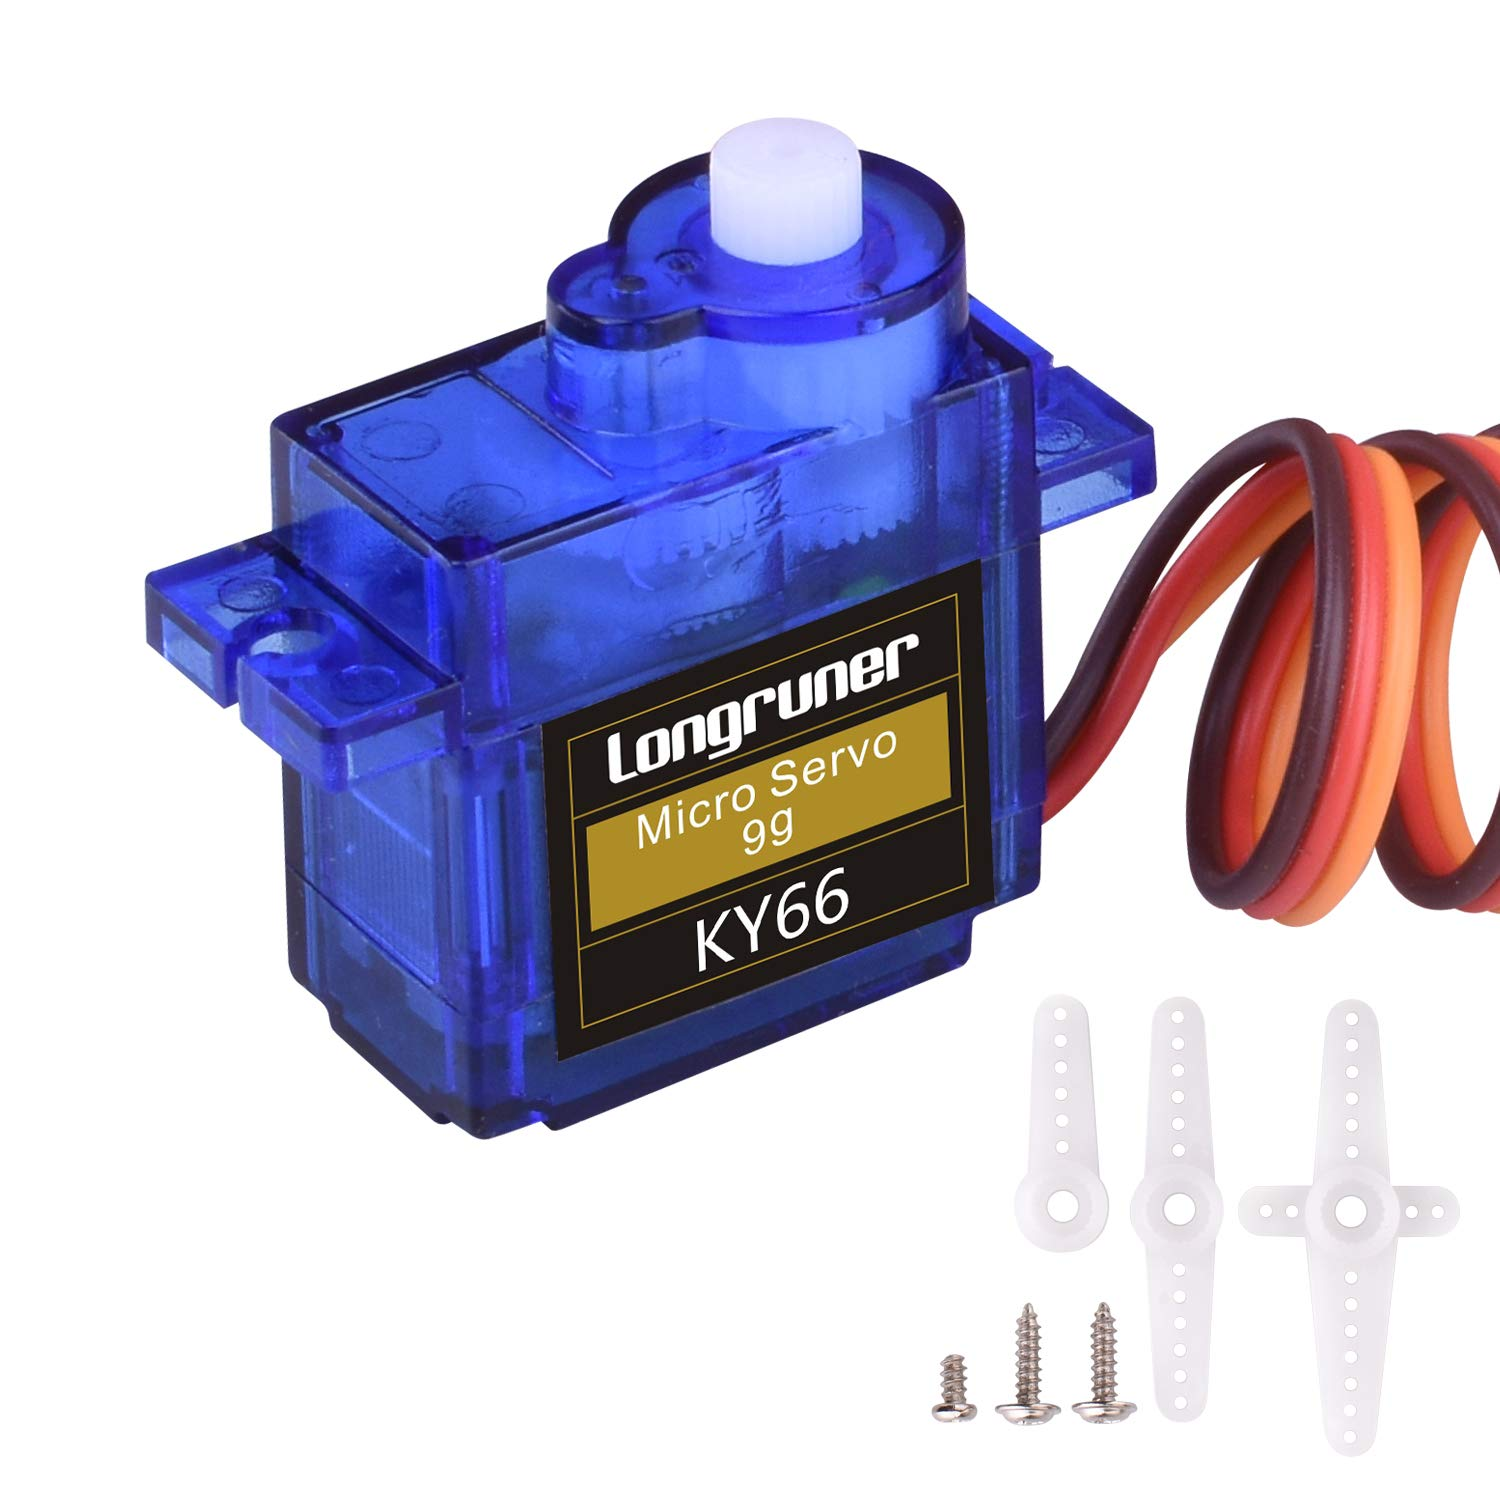
\includegraphics[scale = 0.1]{servo.jpg}
    \caption{Longruner SG90 mini servomoteur 9g \cite{servos} }
    \label{fig:servo}
    \end{minipage}
\end{figure}

Les servomoteurs responsables de la fermeture et inclinaison de la pince sont des mini servos SG90 9g \cite{servos}. Leur vitesse de fonctionnement est de 0,12 sec/60\degree \ et ils possèdent un couple de 1,6kg.cm. Du fait de la légèreté de la pince, ce couple est suffisant pour qu'un servomoteur la soulève (action la plus demandeuse en couple) : la masse de la pince tenant un large tube est de 98g, le bras de levier mesure 13cm, un couple maximal de l'ordre de 1,3kg.cm est donc nécessaire. Les servomoteurs permettent de maintenir la pince dans la position désirée sans qu'il ne soit nécessaire de continuer à les alimenter, et donc risquer de les forcer. Ils sont finalement légers et peu coûteux (\EUR{4}/pièce), ils rentrent donc aisément dans le budget.

La table \ref{recap_moteurs} récapitule les caractéristiques associées à chacun des modèles de moteur.

\vspace{3mm}
\begin{center}
    \begin{tabular}{c | c | c}
    \backslashbox{Caractéristiques}{Type} & Moteurs à encodeurs & Servomoteurs \\ \hline
    Prix & \EUR{8} & \EUR{4} \\ \hline
    Vitesse de rotation & 160 tours/min & 0,12 sec/60\degree \\ \hline 
    Couple & 0,2 kgf.cm &  1,6 kg.cm \\ \hline
    \multirow{2}{*}{Tension} & 3V & 3,0V \\
    & 7,5V & 7,2V \\\hline
    Poids & 50g & 9g
\end{tabular}
\vspace{5mm}
\captionof{table}{\label{recap_moteurs}Caractéristiques moteurs}
\end{center}

\subsection{Microcontrôleur}

Les microcontrôleurs et ordinateurs adaptés au projet, à sa taille et à son budget étaient les Raspberry Pi, Arduino et semblables, de par leur prix bas (de l'ordre de 15-40€), leur puissance de calcul, mémoire et rapidité adaptés aux projets de cette envergure.

Le microcontrôleur Arduino est plus facile à manipuler et est suffisant pour les tâches que le robot doit effectuer. En effet, le robot ne possède pas de caméra et les tâches sont relativement simples en exécution. L'ordinateur \textit{Raspberry Pi}, bien que plus puissant, est plus compliqué à utiliser. Il est également bien plus coûteux.

L'Arduino a été retenu. La version Uno \cite{Arduino_uno} a été choisie, le nombre de pins (20) de cette dernière étant amplement suffisant aux besoins du véhicule. Elle a été préférée à la version Mega \cite{Arduino_mega}, de plus grande taille et comportant 70 pins, mais près de deux fois plus chère, ainsi qu'à la version Due \cite{Arduino_due}, limitée elle à un voltage d’opération de 3,3V (contre 5V pour le Uno), et à la version Nano \cite{Arduino_nano}, de prix inférieur mais de taille inférieure la rendant moins pratique à l'emploi. Un récapitulatif de caractéristiques de ces quatre modèles d'Arduino se trouve dans la table \ref{comp_arduino}.


\begin{figure}[H]
    \begin{minipage}[c]{.46\linewidth}
    \centering
    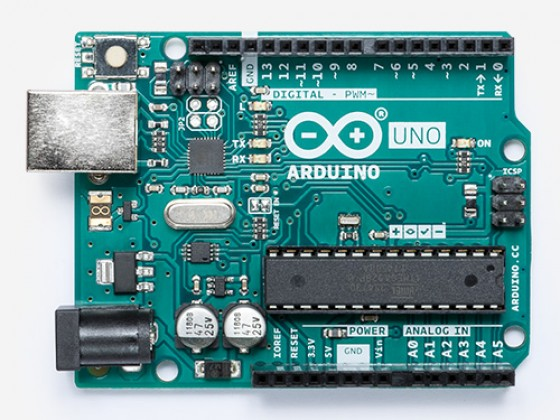
\includegraphics[scale = 0.4]{arduino_uno.jpg}
    \caption{Arduino Uno ayant 14 pins digitales et 6 analogiques \cite{arduno}}
    \label{fig:Uno}
    \end{minipage}
    \hfill
    \begin{minipage}[c]{.46\linewidth}
    \centering
    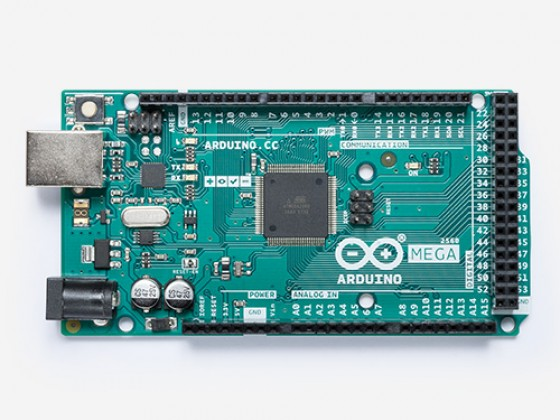
\includegraphics[scale = 0.4]{arduino_mega.jpg}
    \caption{Arduino Mega ayant 54 pins digitales et 16 analogiques \cite{ardmega}}
    \label{fig:Mega}
    \end{minipage}
\end{figure}

\vspace{10}
\begin{center}
    \begin{tabular}{c | c | c | c | c }
    \backslashbox{Caractéristiques}{Modèle} & Uno & Mega & Nano & Due \\ \hline
    Prix & 17\EUR{} & 30\EUR{} & 7.5\EUR{} & 33\EUR{}\\ \hline
    Nombre de pins & 20 & 70 & 26 & 70 \\ \hline 
    Taille & Moyen & Grand & Petit & Grand \\ \hline
    Tension & 5V & 5V & 5V & 3V  \\ \hline
\end{tabular}
\vspace{5mm}
\captionof{table}{\label{comp_arduino}Comparatif des modèles Arduino}
\end{center}

\subsection{Batterie, boîtier de piles}

La batterie utilisée pour alimenter le robot est une Turnigy 1000mAh 3S 20C Lipo Paquet \cite{Lipo}, conseillée par les superviseurs du projet. Sa capacité minimale est de 1000mAh, pour une configuration 3S1P/ 11,1V/ 3Cell. Elle a une masse de 87g et des dimensions de 77*33*20mm. Elle a donc une bonne capacité et l'avantage d'être légère.
Cependant pour éviter d'épuiser excessivement la batterie, un boîtier à piles a été ajouté. Celui-ci est responsable de l'alimentation des moteurs. Il est également plus prudent d'avoir deux sources de tension par mesure de sécurité.

\begin{figure}[H]
    \centering
    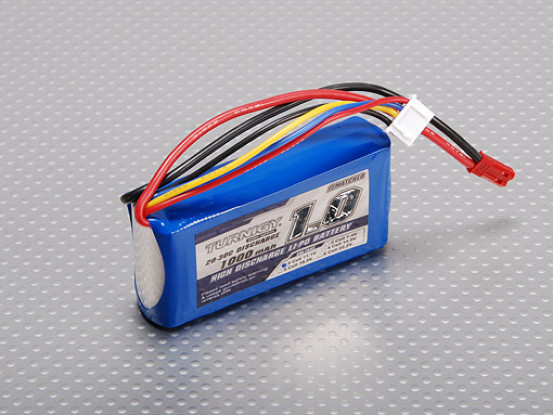
\includegraphics[scale = 0.35]{Lipo.jpg}
    \caption{Batterie Lipo 1000mAh \cite{Lipo}}
    \label{fig:Lipo}
\end{figure}

\subsection{Capteurs\label{capteurs}}

Les capteurs retenus conformément à la stratégie sont deux capteurs Sharp GP2D120X à rayons infrarouges \cite{captdist} fournis par l'École, placés de chaque côté du robot. Les rayons émis sont orientés perpendiculairement à la direction d'avancée du robot pour éviter des éventuelles interférences entres les tubes (l'un entrant dans le cône de détection avant que l'autre n'en soit sorti comme sur la figure \ref{fig:cônedetect}). Les capteurs sont donc placés à la verticale sur le châssis. Les rayons sont émis lorsque le véhicule se meut mais ne sont renvoyés aux capteurs que s'ils ont été réfléchis par un tube. De cette manière le système peut calculer la durée de détection de chaque tube tout en avançant à vitesse constante. Le système associe les périodes de détection les plus courtes aux petits tubes et les plus grandes aux tubes les plus larges. Ainsi les tubes sont triés, et leur position et leur type est gardés en mémoire.

\begin{figure}[H]
    \begin{minipage}[c]{.40\linewidth}
    \centering
    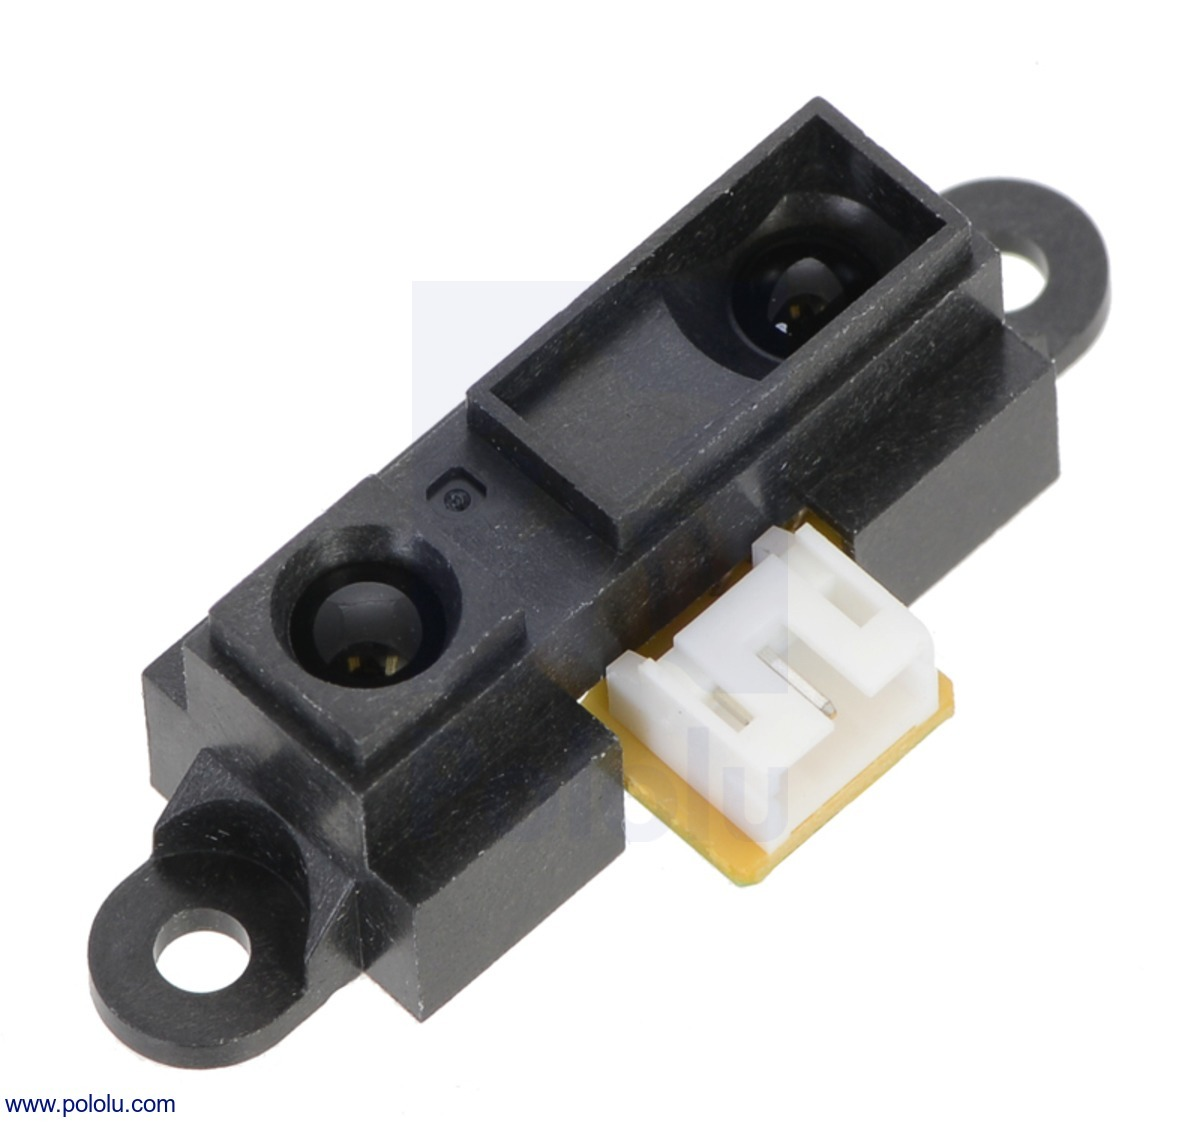
\includegraphics[height = 90]{Capteurs_d.jpg}
    \caption{Capteur de distance : \textit{SHARP GP2D120X} \cite{captdist}}
    \label{fig:captdist}
    \end{minipage}
    \hfill
    \begin{minipage}[c]{.40\linewidth}
    \centering
    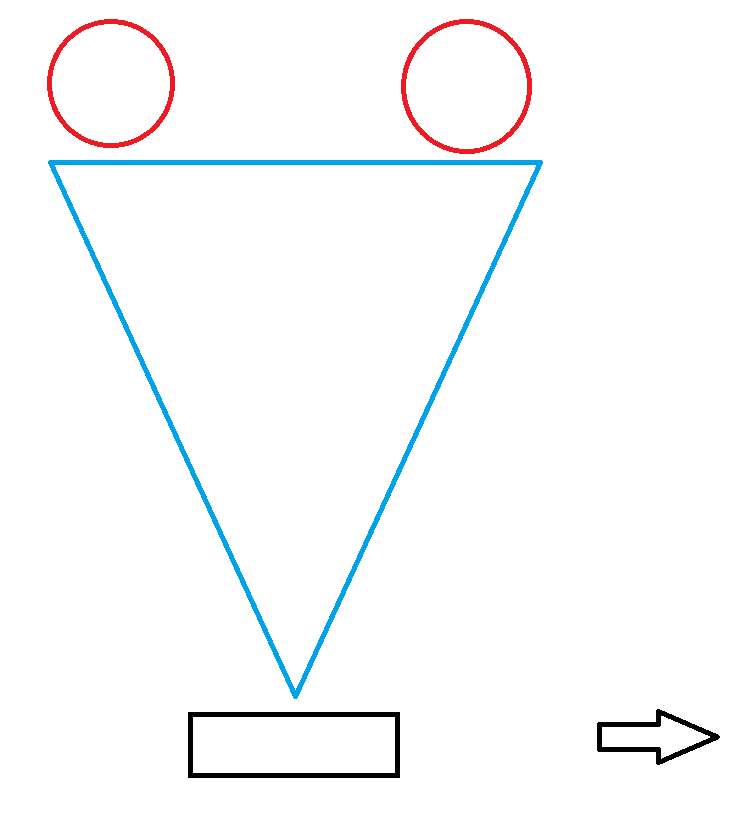
\includegraphics[height = 90]{capteurs_horizontaux.png}
    \caption{cône de détection horizontal}
    \label{fig:cônedetect}
    \end{minipage}
\end{figure}

Toutefois un risque de parasitage reste fréquent avec ce type de capteurs. Cela peut-être le sol qui réfléchit un rayon ou un bruit environnant. La solution choisie est d'encadrer le faisceau avec un cache qui empêche une trop grande dispersion des rayons \cite{Parasites_capteurs_sharp}. En effet les capteurs ont tendance à se disperser et donc perdre en précision à partir d'une certaine distance. C'est pourquoi l'avantage d'un tel dispositif est une précision accrue de la mesure de distance à plus grande portée.

\subsection{Breadboard}
 
Un breadboard sert de support au circuit électronique du robot, sur lequel la plupart des connections sont établies. Il suffit d'y insérer les extrémités des fils électriques, sans avoir recours à de la soudure, ce qui est très pratique pour effectuer des modifications. Cela évite de plus d'avoir à refaire les soudures.

\subsection{H-bridge}

Un H-bridge est nécessaire pour pouvoir contrôler la tension envoyée dans les moteurs. Il permet également de décider du sens de rotation des moteurs.

\section{Construction du robot}

\subsection{Agencement des composants}

\begin{figure}[H]
    \begin{minipage}[c]{.46\linewidth}
        \centering
        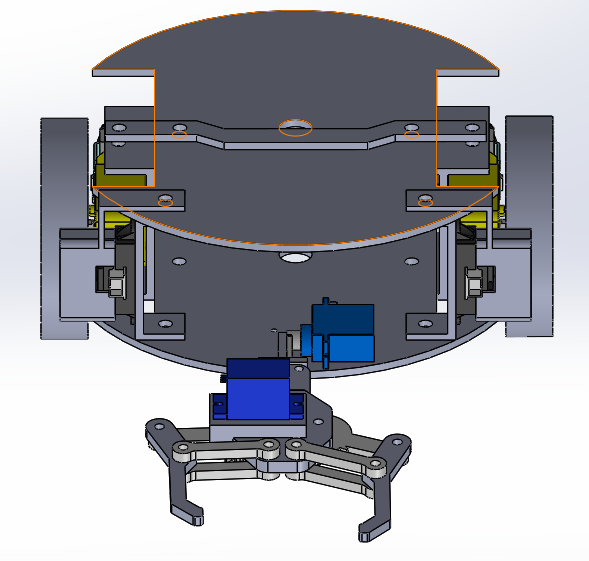
\includegraphics[scale = 0.5]{robot_nu.PNG}
        \captionof{figure}{\label{fig:chasavt}Avant du châssis en vue plongée}
    \end{minipage}
    \hfill
    \begin{minipage}[c]{.46\linewidth}
        \centering
        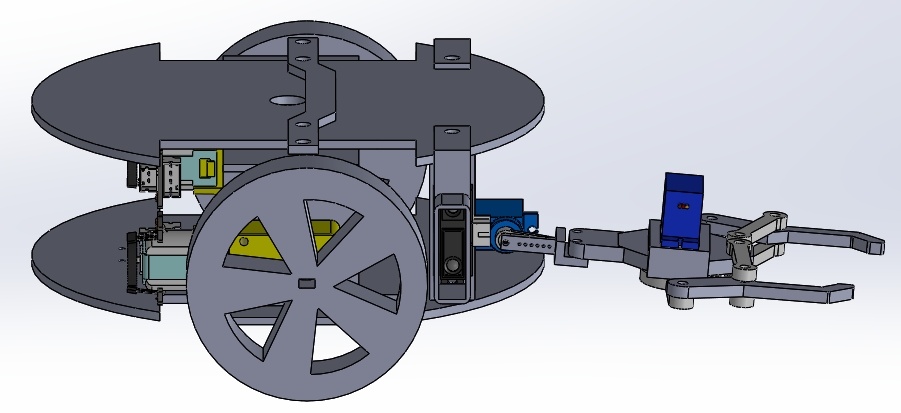
\includegraphics[scale = 0.46]{robot_nu2.PNG}
        \captionof{figure}{\label{fig:chasarr}Côté droit du châssis}
    \end{minipage}
\end{figure}

Sur ce châssis à deux étages (vide de la plupart de ses composants), deux encoches sont prévues pour y insérer les roues. Les câbles d'alimentation et de transmission d'informations entre les composants passent entre ces deux plaques, et sont donc cachés sans risque de frottement quelconque avec les roues ou avec l'environnement extérieur. Les moteurs se situent entre les deux plaques horizontales (figures \ref{fig:chasavt} \& \ref{fig:chasarr}) et sont vissés sur les plaquettes verticales placées au centre du véhicule (liant les deux plaques horizontales). Les roues sont attachées aux moteurs. Les deux plaques sont également fixées entre elles par un ensemble de vis dans des tubes filetés à l'arrière, tandis qu'à l'avant, la plaque du haut est soutenue par d'autres plaquettes verticales (figure \ref{fig:chasavt} page \pageref{fig:chasavt}). Ainsi, le châssis du véhicule tient solidement ensemble et il n'y a aucun jeu lors du mouvement du robot. \newline

\begin{figure}[H]
\centering
    \begin{minipage}[c]{.46\linewidth}
        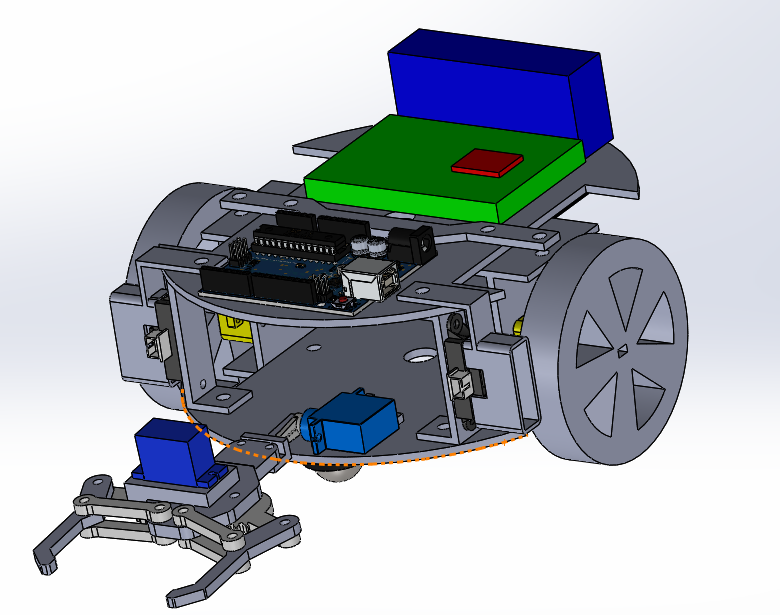
\includegraphics[scale = 0.6]{robot.PNG}
        \captionof{figure}{\label{fig:vehavt}Avant du véhicule en vue plongée avec la pince baissée}
    \end{minipage}
\end{figure}

L'Arduino Uno (en noir sur la figure \ref{fig:vehavt}), la batterie (en bleu à l'arrière du robot) et le breadboard (en vert) sur lequel est positionné le H-Bridge (en rouge), sont les composants principaux et sont placés sur la plaque supérieure. La batterie et le boîtier à piles ont été placés à l'arrière, dans le but de compenser le poids s'exerçant à l'avant du robot du à la pince et à un tube. De plus ces composants principaux ont été disposés de sorte à minimiser la longueur des connections entre ceux-ci. Les capteurs infrarouges se trouvent juste devant les roues sur les côtés du châssis, cachés par des pièces rectangulaires (voir point \ref{capteurs} page \pageref{capteurs}). Les capteurs ont été placés à ces endroits car leur champ de détection doit absolument être orienté latéralement par rapport au robot. La pince est positionnée à l'avant du véhicule et le châssis supérieur est creusé pour permettre à la pince de s'élever. La pince est fixée au châssis via un premier servomoteur (en bleu clair) vissé entre les étages. Le second servomoteur est fixé sur la pince (en bleu marine).

%\subsection{La tortue, le design} % RIP

\newpage
\subsection{Méthodes de construction et matériaux\label{methcstr}}

Après avoir modélisé le châssis sur \textit{SolidWorks}, sa réalisation pouvait se faire en impression 3D ou à la découpe laser. La découpe étant bien plus rapide que l'impression 3D et d'une bonne précision, cette méthode a été privilégiée (voir tableau ci-dessous).

\vspace{3mm}
\begin{center}
    \begin{tabular}{c | c | c}
    \backslashbox{Critères}{Méthodes} & Impression 3D & Découpe \\ \hline
	Temps de fabrication & 10h & 30min\\ \hline
	Précision & Très haute & Bonne \\ \hline
	\multirow{2}{*}{Disponibilité} & Prise de rendez-vous & Prise de rendez-vous \\
	& avec le superviseur ou le Fablab ULB & avec le Fablab ULB\\
\end{tabular}
\vspace{5mm}
\captionof{table}{\label{compimpr}Comparatif de l'impression 3D et de la découpe \bsc{LASER}}
\end{center}

Cependant, les deux plaques ont été premièrement sciées dans une plaque de bois car les découpeuses laser du \textit{fablab} n'étaient pas directement disponibles. De plus, la découpe manuelle était suffisamment précise pour cette application. Elles ont donc été rendues circulaires à l'aide d'une défonceuse. Des trous ont été placés pour permettre de fixer les composants aux endroits nécessaires et de visser les plaques entre elles. Le résultat est très satisfaisant; par conséquent, une découpe plus précise ressortait surtout comme une grande perte de temps. 

Les raccords entre ces deux plaques et d'autres pièces optimisant l'horizontalité du robot ont été imprimées en 3D, tout comme la pince, car ces pièces demandaient un niveau de précision relativement haut de par leur géométrie plus complexe. Afin de pouvoir attraper les tubes de deux diamètres différents en évitant leur glissement, du "griptape" (habituellement utilisé sur le manche des raquettes de tennis) a été placé sur les bras comme matériau antidérapant

Les différents composants se trouvant sur le châssis ont été fixés à l'aide de Velcro.
\clearpage


\section{\label{fonctionnement}Fonctionnement global du robot} %plus indiqué ici

\begin{figure}[H]
    \centering
    \includegraphics[scale = 0.5]{organigramme.png}
    \captionof{figure}{\label{fig:orga} Déroulement de la manipulation. Les actions concrètes ou les données du terrain sont en vert, les éléments physiques du robot en bleu, les concepts théoriques gérés par l'Arduino pour se repérer et se déplacer en orange et enfin l'objectif final en rouge.}
\end{figure}

Premièrement, une consigne de déplacement est envoyée aux moteurs des roues via le H-bridge par l'Arduino, ce qui se traduit par une commande en tension qui correspond au profil de vitesse théorique. Ensuite, l'encodeur optique du moteur renvoit une information à l'Arduino, faisant entrer par après l'odométrie et la régulation en jeu, détaillées respectivement dans les sections \ref{sec:odo} et \ref{sec:reg} pages \pageref{sec:odo} et \pageref{sec:reg}. Celles-ci permettent respectivement au véhicule de connaître sa position sur le plateau et de maintenir la consigne reçue malgré les imperfections de l'environnement, des composants, etc. Une fois le véhicule mis en route, la phase de détection débute.

La première phase est une phase de détection durant laquelle le véhicule avance droit à vitesse constante, après une accélération, pour détecter les tubes via ses capteurs. Les capteurs infrarouges renvoient une information à l'Arduino lorsque leur faisceau est coupé par un tube. L'Arduino s'occupe ensuite de compter le nombre de tics durant lesquels le faisceau est coupé. Les tics correspondent au nombre de fois que la fonction principale est appelée par seconde, il suffit ensuite de les transformer en secondes pour pouvoir déterminer le diamètre du tube détecté. Un petit tube renverra un plus petit nombre de tics qu'un grand car le temps pour le dépasser est plus petit. En plus du temps de détection de chaque tube, l'Arduino va garder en mémoire la position du tube sur le terrain (la position en x est donnée par l'odométrie et celle en y par la distance renvoyée par les capteurs).

La deuxième phase se déroule après la détection de tous les tubes. Le véhicule choisit le tube le plus proche, se tourne vers ce dernier et se déplace jusqu'à lui en ligne droite grâce à la régulation et l'odométrie. Ensuite, le robot ouvre sa pince en contrôlant l'angle des servomoteurs, la fait descendre, attrape le tube et remonte la pince. Une fois le tube soulevé, le robot va se déplacer jusqu'à la zone de dépôt correspondant au type de tube et lâcher ce dernier dans sa zone. Cette phase se déroule 4 fois, afin de déplacer les 4 tubes.
\clearpage

\section{\label{sec:odo}Odométrie}

Comme annoncé à la section \ref{subsec:choix}, puisque le robot ne peut se servir des lignes au sol comme d'un repère permettant de connaître son positionnement en temps réel sur le terrain, il se repère à l'aide d'une odométrie.

Il s'agit d'un module à implémenter au robot pour que celui-ci soit en mesure d'avoir accès à sa position approximative ainsi qu'à son orientation à l'instant même où il en a besoin. Une odométrie cartésienne à deux dimensions (selon les axes x et y) suffit ici étant donné que l'environnement dans lequel évolue le véhicule est une surface plane à l'horizontale. Le raisonnement global du principe d'odométrie est repris par la figure \ref{fig:approx} à la page \pageref{fig:approx}.

La mise en pratique d'un tel système nécessite quelques composants indispensables : des capteurs appelés \textit{encodeurs optiques} qui mesurent le nombre exact de tours réellement effectués par les arbres moteurs, sous forme de tics. Ainsi, sur un intervalle de temps défini, le nombre de tics renvoyé par les encodeurs droit et gauche peuvent être transformé en un déplacement du robot à partir de la résolution des codeuses et de la géométrie du modèle dynamique; tout ceci étant traité par l'Arduino, jouant le rôle de centre d'opérations et de calculs. Ces calculs de position et d'orientation du robot peuvent être réalisés à partir de deux méthodes distinctes.\\\\
\textbf{Approximation par segment de droite:} la trajectoire du robot peut est découpée en déplacements infinitésimaux rectilignes suivant l'orientation précédente.\\
\textbf{Approximation par arc de cercle:} la trajectoire du robot est décomposée en arcs de cercle infinitésimaux.\\

Étant donné que ces deux techniques sont équivalentes si les mesures se font à fréquence suffisamment élevée, la première méthode est préférée (elle nécessite des calculs moins lourds \cite{noauthor_robotics:odometrie_2014}).

A l'instant où l'on a besoin de connaître l'état du robot, c'est-à-dire sa position et son orientation, il s'agit d'abord de récupérer les informations détenues par les encodeurs. Il est ensuite nécessaire de transformer celles-ci en variation de distance et d'angle. Pour ce faire, il faut avoir préalablement déterminé les coefficients théoriques de transformation de distance définissables à partir de la résolution de chacune des codeuses et de la géométrie des roues.

\begin{figure}[H]
    \centering
    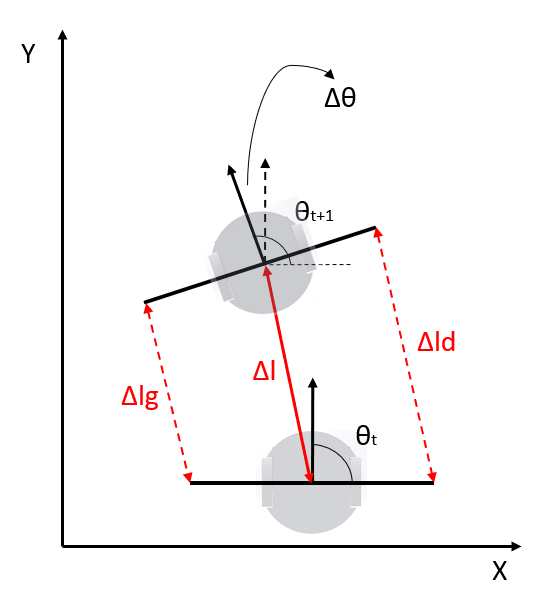
\includegraphics[scale = 0.9]{approxsegment.PNG}
    \caption{Schématisation générale du système d'odométrie}
    \label{fig:approx}
\end{figure}

Sur un intervalle de temps $\Delta$t:\\ \\
Soit les coefficients de transformation de distance $coeff_{D}$ et $coeff_{G}$.\\ 
Soit les informations des encodeurs $x_{tic_{D}}$ et $x_{tic_{G}}$.\\
Soit $\Delta l_{D}$ la variation en terme de distance de la roue droite.\\
Soit $\Delta l_{G}$ la variation en terme de distance de la roue gauche.

\begin{equation*}
    \Rightarrow\left\{
      \begin{aligned}
        \Delta l_{D} & = coeff_{D}*x_{tic_{D}}\\
        \Delta l_{G} & = coeff_{G}*x_{tic_{G}}
        \end{aligned}
    \right.
\end{equation*}\\
Dès lors, les déplacements respectifs des roues donnent accès au déplacement global du robot ainsi qu'à sa nouvelle orientation :
\newpage

\noindent Soit $\Delta l_{moy}$ la distance parcourue par le centre du robot.\\
Soit $\Delta\theta$ la variation d'orientation du robot.\\
Soit L la distance entre les deux roues du robot.

\begin{equation*}
    \Rightarrow\left\{
      \begin{aligned}
        \Delta l_{moy}  & =\frac{\Delta l_{D}+\Delta l_{G}}{2}\\
        \Delta\theta  & = \arctan(\frac{\Delta l_{D}-\Delta l_{G}}{L}) \approx \frac{\Delta l_{D}-\Delta l_{G}}{L}
        \end{aligned}
    \right.
\end{equation*}\\
En ce qui concerne le reste du raisonnement, il faut convertir les variations de distance en déplacements selon l'axe x et l'axe y. Le déplacement étant considéré ici comme un segment de droite, il faut prendre en compte la dernière orientation du robot \cite{noauthor_robotics:odometrie_2014}:\\\\
Soit $\theta_{t-1}$ l'orientation obtenue à la dernière mesure

\begin{equation*}
    \Rightarrow\left\{
      \begin{aligned}
        \Delta x = \Delta l*\cos(\theta_{t-1})\\
        \Delta y = \Delta l*\sin(\theta_{t-1})
        \end{aligned}
    \right.
\end{equation*}

Pour finir, le calcul de la position et de l'orientation du robot à l'instant présent se fait comme suit:
\begin{equation*}
    \Rightarrow\left\{
      \begin{aligned}
        x_{t} = x_{t-1} + \Delta x\\
        y_{t} = y_{t-1} + \Delta y\\
        \theta_{t} = \theta_{t-1} + \Delta\theta\\
        \end{aligned}
    \right.
\end{equation*}\\

Dès lors, le bloc odométrie permet à n'importe quel moment de sortir un triple ($x_{t}$, $y_{t}$, $\theta_{t}$) correspondant à l'état du robot à cet instant précis, c'est-à-dire respectivement sa coordonnée selon x, sa coordonnée selon y et son orientation. Par ailleurs, les approximations faites ci-dessus sont assez grossières et peuvent ainsi induire une dérive considérable sur de longs trajets, c'est pourquoi la fréquence de mesure doit être assez élevée afin que les déplacements pris en compte apparaissent comme étant infinitésimaux, préservant la validité de l'approximation par segment de droite.
\clearpage

\section{\label{sec:reg}Régulation}

Maintenant que le robot a accès à sa position ainsi qu'à son orientation en temps réel tandis qu'il évolue dans son environnement, il est envisageable de lui imposer un déplacement d'un endroit à un autre en lui donnant uniquement comme consigne un couple de coordonnées cartésiennes correspondant à la destination voulue.

\subsection{Objectif}

Pour réaliser la stratégie mise en place, il faut donner au robot des consignes de position adaptées qu'il mettra en oeuvre au moment voulu grâce à un déplacement précis et contrôlé. C'est ici qu'intervient la régulation en terme de position. Approchons-la intuitivement.

Prenons par exemple la manoeuvre de base qu'est "\textit{rouler en ligne droite}". En toute logique, la toute première intuition serait d'appliquer des tensions identiques aux moteurs droit et gauche. la solution n'est malheureusement pas si simple. En effet, le problème est qu'en réalité, le robot va être confronté à des imperfections imprévisibles telles que des frottements secs au sein des moteurs, ou encore des différences de fabrication entre les moteurs censés être similaires. Celles-ci fausseront donc le déplacement réellement effectué par le robot. En d'autres termes, elles lui feront dévier de son objectif.

C'est pourquoi il est nécessaire de mettre en place un système de régulation permettant au véhicule de prendre en compte les erreurs entre la consigne à effectuer et ce qu'il en est réellement. Ce pour pouvoir minimiser cette erreur, voir potentiellement l'annuler, en rectifiant le comportement du robot au cours du temps. La régulation PID, pour \textit{Proportionnelle}, \textit{Intégrale} et \textit{Dérivée}, est l'une des méthodes les plus utilisées au sein des processus industriels \cite{le_lann_pid_2007}. Elle permet, comme expliqué ci-dessus, d'atteindre et de maintenir un paramètre quelconque aussi près que possible de la consigne demandée, le tout en boucle fermée comme le montre la figure \ref{fig:boucle}. Pour ce faire, l'erreur sur la consigne doit être calculée à intervalles réguliers (pour plus de stabilité) et à l'aide de capteurs adaptés. Elle est ensuite exploitée sous différentes formes de manière à obtenir un système asservi ayant le comportement souhaité. Les traitements que subit l'erreur se font en faisant intervenir dans les asservissements proportionnel, intégral et dérivée, respectivement, l'erreur de base, la somme totale des erreurs ainsi que la différences des deux dernières erreurs mesurées. L'effet que ces différents termes ont sur le comportement du robot sera détaillé dans la sous-section \ref{subsec:influence} page \pageref{subsec:influence}.

\subsection{\label{ptregpos}Régulation de position}

Le but étant de déplacer le robot d'un endroit à un autre le plus rapidement possible, la régulation est faite sur la position du robot. La consigne que le robot reçoit est un couple de coordonnées cartésiennes correspondant à l'endroit où il doit se rendre sur la carte.

Cette consigne principale est ensuite divisée en deux sous-consignes correspondant aux blocs en turquoise sur la figure \ref{fig:boucle}, une consigne de distance $l_{consigne}$ et une consigne d'angle $\theta_{consigne}$, par calculs faisant intervenir des notions vectorielles et trigonométriques. Chacune de ces deux consignes constantes est décomposée en une succession de consignes évolutives afin d'avoir un contrôle du déplacement à tout instant et non pas exclusivement sur le résultat final. C'est par rapport à ces consignes évolutives que les erreurs d'angle et de distance sont finalement calculées.

Pour ce faire, l'état du robot à un instant donné est récupéré par le biais du bloc odométrie, en orange sur la figure \ref{fig:boucle}, avant d'être comparé à l'état dans lequel il est supposé être. Ces erreurs rentrent alors dans les blocs d'asservissement, en vert sur la figure \ref{fig:boucle}, desquels ressortent les commandes en tensions qui minimisent l'erreur sur chacune des consignes à réguler. Ces commandes sont finalement appliquées au moteur droit et au moteur gauche en suivant la logique des vitesses différentielles, le tout en tenant compte des caractéristiques utiles des moteurs par l'ajout des tensions minimales respectives, "\textit{Uo\_D}"  et  "\textit{Uo\_G}", pour lesquelles les moteurs entrent en action.

\begin{figure}[H]
    \centering
    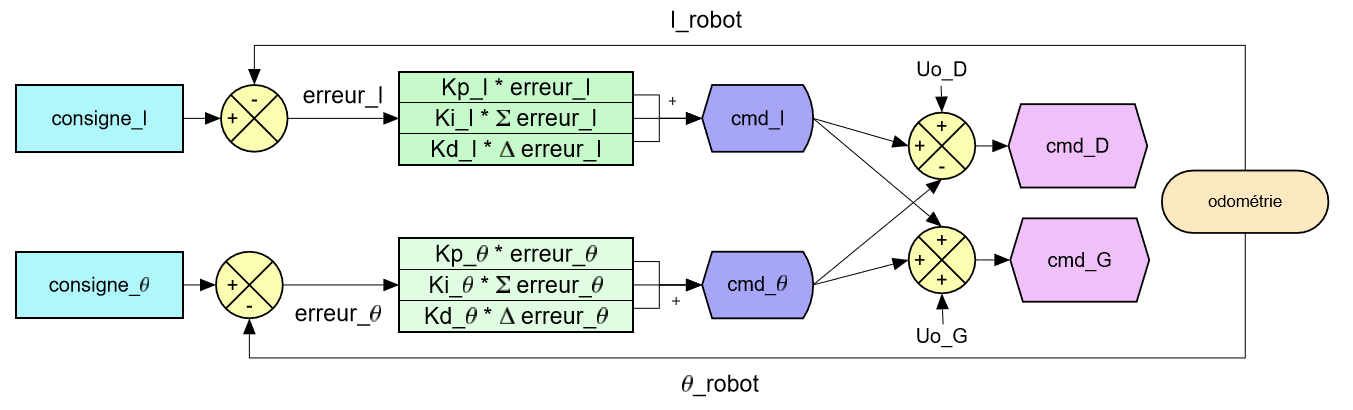
\includegraphics[scale = 0.55]{Capture.PNG}
    \caption{Boucle d'asservissement de position}
    \label{fig:boucle}
\end{figure}

\subsubsection{\label{subsubsec:sous}Calcul des deux sous-consignes}

Le raisonnement suivant est fait selon un système de coordonnées cartésiennes dont les axes x et y suivent respectivement la largeur et la longueur de la carte, et selon une orientation suivant le système trigonométrique. La distance à parcourir par le robot s'obtient en calculant la norme du vecteur construit par ses deux points extrêmes. Le calcul de l'angle à effectuer par le robot pour se trouver en face de sa cible utilise la fonction atan2(y,x), fonction à 2 variables permettant en pratique de trouver l'angle entre l'axe des x positifs et la droite passant par l'origine (0,0) et par le point (x,y) \cite{cochelin_positionnement_nodate} (comme le montre la figure \ref{fig:atan} ci-dessous).

\begin{figure}[H]
    \centering
    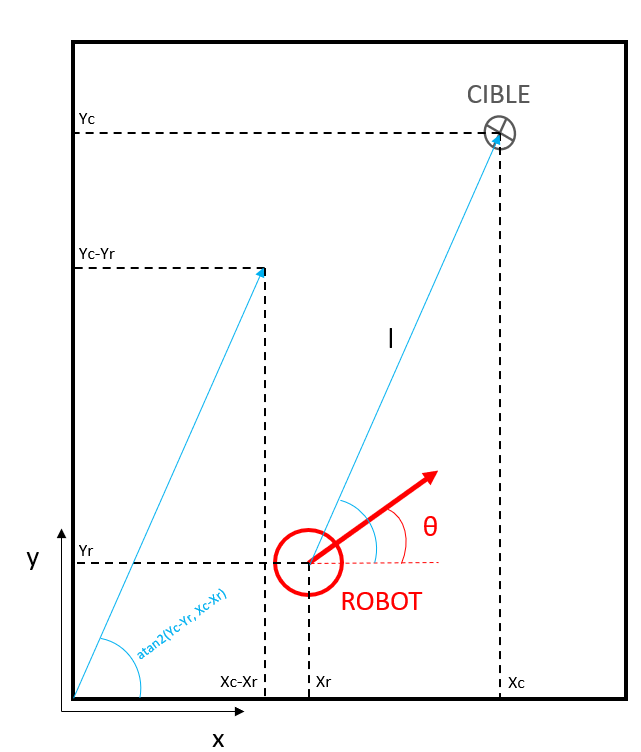
\includegraphics[scale = 0.75]{atan2.PNG}
    \caption{Représentation graphique du calcul des consignes}
    \label{fig:atan}
\end{figure}\\

A l'instant t où le robot reçoit une consigne:\\
Soit la position cible ($x_{cible}$, $y_{cible}$).\\
Soit l'état du robot à cet instant (x, y , $\theta$).

\begin{equation*}
    \Rightarrow\left\{
        \begin{aligned}
            l_{consigne} & = \sqrt{(x_{cible}-x)^2+(y_{cible}-y)^2}\\ 
            \theta_{consigne_{rad}} & = atan2(y_{cible}-y, x_{cible}-x)-\theta
        \end{aligned}
    \right.
\end{equation*}\\
Avec $\theta_{consigne_{rad}}$ compris entre -$\pi$ et $\pi$ radian\\\\
\begin{equation*}
    \Rightarrow\left\{
        \begin{aligned}
            \theta_{consigne_{deg}} = l_{consigne_{rad}}*\frac{180}{\pi}
        \end{aligned}
    \right.
\end{equation*}\\
Avec $\theta_{consigne_{deg}}$ maintenant compris entre -180$\degree$ et 180$\degree$.

\subsubsection{\label{evo}Consignes évolutives}

A ce stade-ci, il s'agit de décomposer les deux sous-consignes pour éviter le problème suivant. En demandant au robot de se rendre à un point cible de son environnement, seul le résultat final est contrôlé par la boucle d'asservissement (voir figure \ref{fig:boucle} page \pageref{fig:boucle}), et le comportement du robot en terme de vitesse tout au long de son déplacement n'est pas considéré. Cela devient problématique car au delà d'une certaine distance courte à parcourir, le robot fait tourner ses moteurs à plein régime sans adapter sa vitesse, ce qui mène à une perte de contrôle inévitable. De plus, cela pourrait endommager irréversiblement les moteurs.

Pour pallier à ce problème, il faut implémenter au robot une consigne qui évolue au cours du temps et qui engendre une vitesse de déplacement bien précise chez le robot. Ainsi, la consigne demandée permet de contrôler l'évolution du mouvement effectué par le véhicule pour aboutir au résultat voulu. L'objectif est d'obtenir un robot se déplaçant - dans la mesure du possible - avec un profil de vitesse trapézoïdal, représenté sur la figure \ref{fig:trapèze}. En d'autres termes, il s'agit de contraindre la puissance délivrée aux moteurs afin que n'importe quelle course ordonnée par une consigne position passe par 3 phases successives bien déterminées : une phase d'accélération constante, suivie d'une phase à vitesse constante, elle-même suivie d'une phase de décélération constante. Le développement suivant reprend le raisonnement permettant d'atteindre une telle ligne de conduite.

\begin{figure}[H]
    \centering
    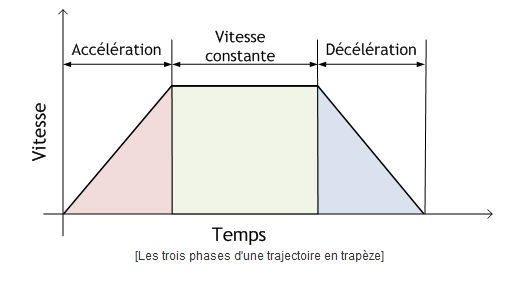
\includegraphics[scale = 1]{Profile_trapeze.png}
    \caption{Profil de vitesse trapézoïdal \cite{noauthor_construction_nodate}}
    \label{fig:trapèze}
\end{figure}

Le calcul du temps $\tau$ que met le robot pour atteindre sa vitesse de croisière se fait simplement comme suit:
\newline

\noindent Soit A l'accélération pour la phase d'accélération constante.\\
Soit $A_{max}$ l'accélération maximale du robot.\\
Soit V la vitesse de croisière pour la phase à vitesse constante.\\
Soit $V_{max}$ la vitesse maximale du robot.
\begin{equation*}
    \left\{
        \begin{aligned}
            A & = \frac{V}{\tau} \Rightarrow \tau = \frac{V}{A}  & (1)\\ 
           \end{aligned}
    \right.
\end{equation*}

La distance parcourue par le robot sur cette phase d'accélération est également la distance parcourue lors de la phase de décélération. Il s'agit de l'aire sous la pente positive du trapèze, c'est-à-dire la zone triangulaire rouge sur la figure \ref{fig:trapèze}.

\begin{equation*}
    \Rightarrow\left\{
        \begin{aligned}
        l_{\tau} & = \frac{A}{2}*\tau^2\\
           \end{aligned}
    \right.
\end{equation*}\\
En substituant $\tau$ par son expression trouvée en (1), on obtient:
\begin{equation*}
    \Rightarrow\left\{
        \begin{aligned}
        l_{\tau} = \frac{V^2}{2A}\\
           \end{aligned}
    \right.
\end{equation*}

À ce stade du raisonnement, il faut prendre en considération deux cas particuliers face auxquels peut se retrouver le robot lorsqu'une consigne lui est imposée. En effet, si la consigne de distance est plus petite que la distance parcourue lors de la phase d'accélération, il paraît évident que le robot ne pourra atteindre sa vitesse de croisière. Dans ce cas, le profil de vitesse devient un profil triangulaire parfois dit profil "bang-bang" \cite{chemori_generation_nodate}.\\

\underline{Si $consigne_{l}$ $\leq$ l_{$\tau$}}:\\

Le fait que la distance parcourue lors de la phase d'accélération est la même que celle parcourue lors de la phase de décélération donne accès au temps $\tau_{bang}$ durant lequel le robot doit accélérer:
\begin{equation*}
    \Rightarrow\left\{
        \begin{aligned}
        \frac{consigne_{l}}{2} = \frac{A*\tau_{bang}^2}{2} \Leftrightarrow \tau_{bang} = \sqrt{\frac{consigne_{l}}{A}}\\
           \end{aligned}
    \right.
\end{equation*}\\
Le mouvement sur la distance aura donc un temps de réalisation global T = 2*$\tau_{bang}$ = $2\sqrt{\frac{consigne_{l}}{A}}$. La fonction continue qui fournit la $consigne_{l_{evo}}$ à transmettre au robot pour générer chez lui un profil de vitesse triangulaire se construit comme suit:
\begin{equation*}
    \left\{
        \begin{aligned}
        l_{evo}(t) & = \frac{A}{2}*t^2 &si t<\tau_{bang}\\
        l_{evo}(t) & = \frac{-A}{2}*(t-\tau_{bang})^2 + (\tau_{bang}*A) *( t-\tau_{bang}) + l_{\tau_{bang}} &si t>\tau_{bang}
        \end{aligned}
    \right.
\end{equation*}

\underline{Si $consigne_{l}$ $>$ $l_{\tau}$}:\\

La distance $l_{\tau}$ parcourue le temps d'atteindre la vitesse de croisière ayant déjà été calculée, il ne reste plus qu'à mesurer la distance à parcourir durant la phase à vitesse constante pour pouvoir accéder au temps de croisière ainsi qu'au temps global d'exécution.

\begin{equation*}
    \left\{
        \begin{aligned}
        l_{V_{cste}} &= consigne_{l} - 2l_{\tau}  = l - \frac{v^2}{A}\\
        t_{V_{cste}} &= \frac{l_{v_{cste}}}{V}  = \frac{A*l-v^2}{AV}\\
        \end{aligned}
    \right.
\end{equation*}\\
\begin{equation*}
    \left.
        \begin{aligned}
        \Rightarrow T = 2\tau + t_{v_{cste}}  = 2\tau + \frac{A*l-V^2}{AV}
        \end{aligned}
    \right.
\end{equation*}\\
Dès lors, la fonction continue de la consigne sur la distance en fonction du temps peut être créée. Celle-ci générant cette fois un profil trapézoïdal de vitesse pour le robot.
\begin{equation*}
    \left\{
        \begin{aligned}
        l_{evo}(t) & = \frac{A}{2}*t^2 &si&: 0<t<\tau\\
        l_{evo}(t) & = V*(t-\tau) + l_{\tau} &si&: \tau<t<T-\tau\\
        l_{evo}(t) & = \frac{-A}{2}*(t-t_{v_{cste}}-\tau)^2 + V*(t-t_{v_{cste}}-\tau) + l_{v_{cste}} + l_{\tau} & si&: T-\tau < t < T
        \end{aligned}
    \right.
\end{equation*}\\
Maintenant que la fonction génératrice des distances est définie, il s'agit de mettre en place la même démarche pour la consigne sur l'angle. Par ailleurs, ces fonctions doivent être évaluées aux moments propices. En pratique, cela se fait à la fréquence d'échantillonnage de l'asservissement. Bien évidemment, il faut toujours avoir une consigne d'avance, c'est-à-dire que la commande ne dit pas au robot où il est mais bien là où il devrait être.
Si f est la fréquence d'échantillonnage à laquelle s'exécute la régulation PID, cela implique que la période échantillonnage équivaut à $\frac{1}{f}$, ce qui correspond à l'intervalle de temps entre deux itérations. Les fonctions de consignes s'évaluent donc suivant ce modèle.\\
\underline{Si i\textsuperscript{ème} itération} :
\begin{equation*}
    \Rightarrow\left\{
        \begin{aligned}
        consigne_{l_{evo}} = l_{evo}(\frac{1}{f}*(i+1))
        \end{aligned}
    \right.
\end{equation*}

La méthode de décomposition de la consigne d'angle en consignes évolutives est rigoureusement similaire à ce qui a été présenté ci-dessus une fois l'accélération linéaire et la vitesse linéaire ayant été respectivement remplacées par l'accélération angulaire et la vitesse angulaire; elle ne sera donc pas détaillée en plus au sein de cette section.

\subsubsection{Calcul des erreurs et asservissements}
Maintenant que les fonctions génératrices des consignes évolutives ont été construites, il s'agit de calculer l'erreur de distance et d'angle, respectivement $erreur_{l}$ et $erreur_{\theta}$, afin d'utiliser celles-ci dans le bloc d'asservissement. Pour ce faire, il faut récupérer le triple (x, y, $\theta$) à la fréquence d'échantillonnage afin d'avoir une erreur qui évolue avec l'état du robot.\\\\
Soit ($x_{0}$, $y_{0}$, $\theta_{0}$) l'état du robot à l'instant où il a reçu la consigne.\\
Soit (x(t), y(t),$\theta$(t)) l'état du robot à l'instant t où l'erreur doit être calculée.\\
Soit $l_{evo}$ la consigne de distance évolutive correspondant à l'instant t.\\
Soit $\theta_{evo}$ la consigne d'angle évolutive correspondant à l'instant t.

\begin{equation*}
    \left\{
        \begin{aligned}
            erreur_{l} & = l_{evo} - \sqrt{(x(t)-x_{0})^2+(y(t)-y_{0})^2}\\
            \Sigma_{erreur_{l}} +&= erreur_{l}\\
            \Delta_{erreur_{l}} & = erreur_{l} - erreur_{l_{old}}\\
            erreur_{l_{old}} & = erreur_{l}\\
            \end{aligned}
    \right.
\end{equation*}

\begin{equation*}
    \Rightarrow commande_{l} =  Kp_{l}*erreur_{l}+Ki_{l}*\Sigma_{erreur_{l}}+Kd_{l}*\Delta_{erreur_{l}}
\end{equation*}

\begin{equation*}
    \left\{
        \begin{aligned}
            erreur_{\theta} & = \theta_{evo} - \theta(t)\\
            \Sigma_{erreur_{\theta}} +&= erreur_{\theta}\\
            \Delta_{erreur_{\theta}} & = erreur_{\theta} - erreur_{\theta_{old}}\\
            erreur_{\theta_{old}} & = erreur_{\theta}\\
        \end{aligned}
    \right.
\end{equation*}

\begin{equation*}
    \Rightarrow commande_{\theta} = Kp_{\theta}*erreur_{\theta}+Ki_{\theta}*\Sigma_{erreur_{\theta}}+Kd_{\theta}*\Delta_{erreur_{\theta}}
\end{equation*}

Le châssis choisi étant fixe, il faut appliquer des vitesses différentielles pour effectuer un changement de direction. C'est pourquoi la commande d'angle doit contribuer positivement pour l'un des moteurs et négativement pour l'autre. On parle d'asservissement différentiel, parfois également appelé asservissement polaire ou en alpha-delta \cite{rouviere_asservissement_2007}.

\begin{equation*}
    \Rightarrow\left\{
        \begin{aligned}
           commande_{moteur_{droit}} & = commande_{l} - commande_{\theta}\\
           commande_{moteur_{gauche}} & = commande_{l} + commande_{\theta}
           \end{aligned}
    \right.
\end{equation*}

Pour finir, il faut s'assurer que les tensions finales correspondant aux commandes à envoyer aux moteurs droit et gauche ne dépassent pas les valeurs nominales de ceux-ci. Il faut également rajouter aux commandes finales les tensions minimales respectives $U_{0_{D}}$ et $U_{0_{D}}$ des moteurs, étant donné que c'est au-dessus de celles-ci que les moteurs font se déplacer le robot. Cela permet ainsi d'obtenir une réactivité optimale de la part du système. Les commandes finales sont :

\begin{equation*}
    \Rightarrow\left\{
        \begin{aligned}
           commande_{moteur_{droit}} & = commande_{l} - commande_{\theta}+U_{0_{D}}\\
           commande_{moteur_{gauche}} & = commande_{l} + commande_{\theta}+U_{0_{G}}
           \end{aligned}
    \right.
\end{equation*}

Ce sont ces commandes calculées par régulation qui seront employées pour alimenter les moteurs au cours de chacun des déplacements.

\subsection{\label{subsec:influence}Influence des coefficients \cite{le_lann_pid_2007}}

La régulation proportionnelle engendre, une commande directement proportionnelle à l'erreur commise. Son but est d'amplifier de manière fictive cet écart afin d'en augmenter la correction réelle, rendant ainsi le système plus vif. En d'autre termes, le coefficient de proportionnalité Kp rend l'erreur plus grande que ce qu'elle n'est vraiment, diminuant ainsi le temps de montée en régime du système. C'est la partie la plus intuitive de la régulation de position : plus le robot est loin de sa cible, plus la puissance délivrée aux moteurs est élevée. De la même manière, plus le robot se rapproche de sa cible, plus la puissance délivrée aux moteurs est faible.

La régulation intégrale vient compléter l'erreur statique laissée par la partie proportionnelle. En effet, une fois la consigne presque atteinte, la commande résultante en tension est trop faible pour actionner les moteurs. Dès lors, le terme intégral prend en compte l'accumulation des erreurs mesurées tout au long des corrections établies pour atteindre l'objectif. Par conséquent, contrairement au terme proportionnel, le coefficient intégral Ki garde un effet stable sur la commande, et ce même lorsque l'écart est minime. Il faut donc faire attention à ne pas trop élever la valeur de celui-ci pour éviter des dépassement trop importants de la consigne désirée, qui entraîneraient des oscillations indésirables autour de la valeur cible.

Le terme dérivé influence quant à lui la commande finale en tenant compte de la différence entre les deux dernières erreurs successives. Cela signifie en pratique qu'il permet d'anticiper quand sera atteinte la consigne en considérant la vitesse à laquelle évolue l'erreur. Effectivement, plus le robot s'approche rapidement de la cible, moins la commande liée au terme dérivé délivre de la puissance - et inversement. Cet élément de régulation s'oppose donc directement à l'effet du coefficient de proportionnalité. Son rôle est majeur lorsque le robot est sur le point d'atteindre sa cible car, tandis que le terme proportionnel est presque nul et que le terme intégral continue d'actionner le système, le coefficient dérivé permet de freiner le robot, diminuant ainsi les oscillations ainsi que le temps de stabilisation de celui-ci.

\subsection{Détermination des coefficients \cite{le_lann_pid_2007}}

Il faut désormais déterminer les valeurs des coefficients intervenant dans le bloc d'asservissement afin d'obtenir un robot qui se comporte et se déplace de manière stable, précise et rapide. La technique la plus fine pour ce faire serait de modéliser l'entièreté du modèle dynamique de notre robot, ce qui n'est pas réalisable à l'échelle du projet étant donné que certains paramètres ne sont pas accessibles. Effectivement, que ce soient les défauts de fabrications, les frottements secs ou encore le jeu au sein des moteurs, aucun de ces paramètres ne peut être parfaitement pris en compte, ce qui rend cette étude mathématique impossible. Il faut donc adopter une démarche empirique, basée sur des tests d'\textit{essais-erreurs}, jusqu'à ce que le comportement du robot satisfasse les attentes de l'équipe.
\newline

Généralement, le robot est voulu le plus précis possible pour une régulation de position, l'erreur statique doit donc être minimale (quitte à perdre en rapidité d'exécution).
Ici, une régulation proportionnelle et dérivée suffit, étant donné que la considération des valeurs de tensions minimales d'action des moteurs ($U_{0}$) remplace la contribution intégrale pour compléter l'erreur statique.

\subsection{\label{subsec:phases}Découpe du déplacement en deux phases}

Cette sous-section présente la façon dont le déplacement du robot vers un point cible est séquencé.

Jusqu'ici le robot régule simultanément une consigne d'angle et une consigne de distance correspondant à une position bien précise à atteindre. En réalité, le robot commence par réguler la consigne angulaire dans une phase de rotation sur lui-même pour ensuite réguler la consigne de distance dans une phase de déplacement rectiligne (il se tourne vers sa cible avant de s'y rendre en ligne droite). Ce découpage du mouvement a pour objectif de séparer partiellement la boucle d'asservissement (figure \ref{fig:boucle}) vue au point \ref{ptregpos} page \pageref{ptregpos} en deux boucles simplifiées ne faisant apparaître qu'un seul bloc. Ainsi, les bloc ne s'influencent plus l'un l'autre, ce qui facilite les réglages.

\subsubsection{Phase de rotation}

Durant cette phase, seule la consigne d'angle évolutive est régulée de manière à ce que le robot s'oriente vers sa cible. La boucle d'asservissement correspondant à cette étape est la suivante.

\begin{figure}[H]
    \centering
    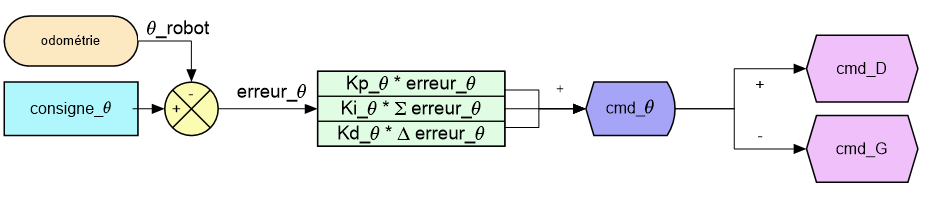
\includegraphics[scale = 0.8]{Captureboucletheta.PNG}
    \caption{Boucle d'asservissement angulaire}
    \label{fig:boucletheta}
\end{figure}

\subsubsection{Phase de déplacement rectiligne}

Cette phase est quant à elle un peu plus complexe. Durant celle-ci est régulé le fait d'avancer droit sur une distance voulue, c'est-à-dire que la consigne de distance vaut \textit{l} tandis que la consigne d'angle est l'angle atteint par la phase de rotation. Par conséquent, la contribution de la régulation sur \textit{l} est beaucoup plus important que celle sur \textit{$\theta$}. La boucle d'asservissement de la figure \ref{fig:boucle} est donc encore assez valide, et la boucle l'approchant correspond à la figure suivante, d'où la séparation partielle annoncée au premier paragraphe de la sous-section \ref{subsec:phases}.

\begin{figure}[H]
    \centering
    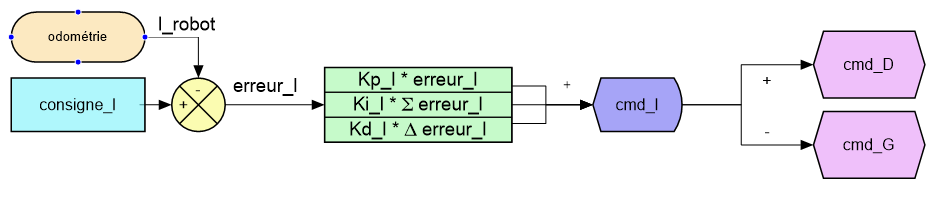
\includegraphics[scale = 0.8]{Capturebouclel.PNG}
    \caption{Boucle d'asservissement de distance}
    \label{fig:bouclel}
\end{figure}
\clearpage

\section{Les simulations}

Deux sortes de simulations ont été mises en place afin de pouvoir tester les différents principes de fonctionnement du robot avant la fin de sa construction. La première, plus axée sur un support graphique, met en évidence la stratégie choisie pour accomplir la mission imposée (voir section \ref{sec: desc} page \pageref{sec: desc}). La seconde a été mise en oeuvre pour mettre à l'épreuve la partie mathématique de la régulation assurant les déplacements du robot.

\subsection{Simulation PyGame}

Cette simulation a eu pour but de tester les stratégies possibles et de les comparer afin de choisir la plus adaptée au projet. Pour cela, le véhicule a été modélisé à échelle, ainsi que son déplacement et que les contraintes inhérentes à tout déplacement dans la réalité (accélération au démarrage, inertie, ...). Elle a été codée sur \textit{Python} via le module \textit{Pygame} \cite{pyginf}. Il s'agit d'un module graphique open source souvent utilisé pour le jeu vidéo \cite{pygjeu} (dû à sa puissance et sa richesse) et parfaitement adaptée pour programmer une simulation purement graphique.

\begin{figure}[H]
    \centering
    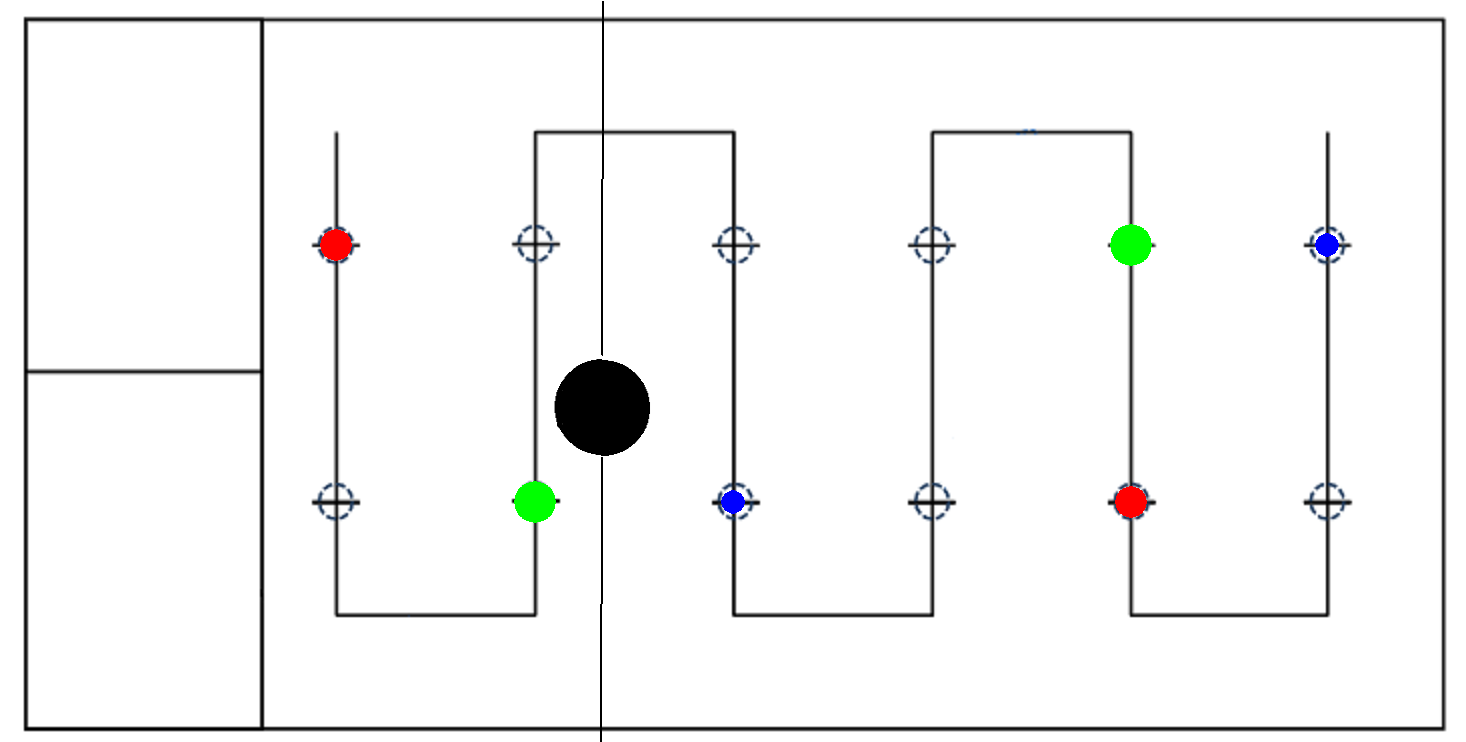
\includegraphics[scale = 0.2]{simu_cyl.png}
    \captionof{figure}{Simulation du véhicule se mouvant sur le terrain.}
    \label{vehmouv}
\end{figure}

La simulation consiste en une fenêtre reproduisant le terrain sur lequel le véhicule se déplace, comme illustré sur la figure \ref{vehmouv}. Un objet "véhicule" interagit avec son environnement. Il est modélisé par une boule noire, tandis que les lignes sur les côtés du véhicule représentent les capteurs infrarouges situés de part et d'autre du robot. Les boules bleues, rouges et vertes correspondent respectivement aux tubes de petit, moyen et grand diamètre.
 
Une loi inertielle est simulée pour rendre la simulation plus réaliste. Elle est imitée en obligeant le véhicule à accélérer progressivement et est également appliquée à la décélération. Une vitesse maximale a été fixée à $0.5m/s$ car le robot est limité à une vitesse de cet ordre. De même, une accélération maximale a été imposée à $1m/s^2$.
 
\begin{figure}[H]
    \begin{minipage}[c]{.46\linewidth}
        \centering
        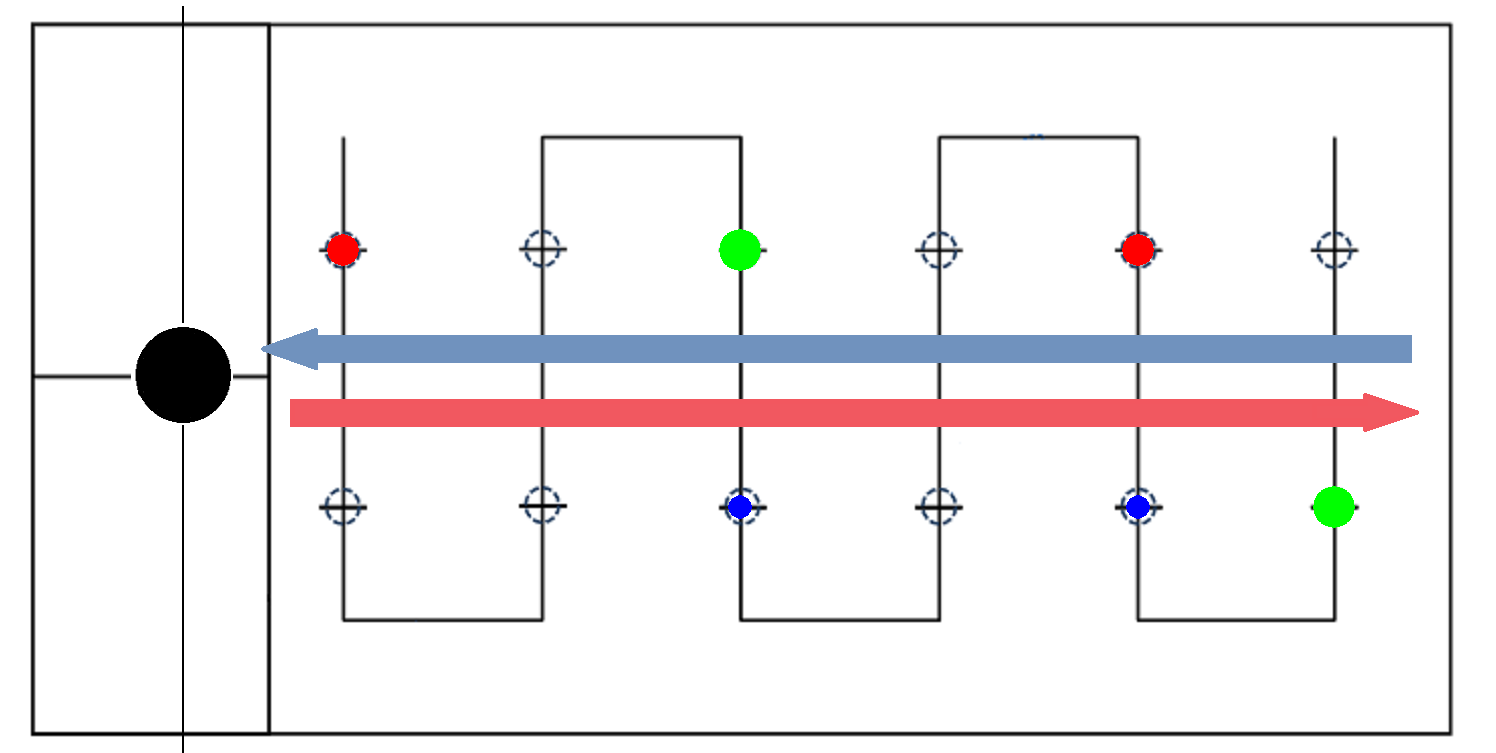
\includegraphics[scale = 0.15]{simu_veh.png}
        \caption{Phase 1 : détection}
    \end{minipage}
    \hfill
    \begin{minipage}[c]{.46\linewidth}
        \centering        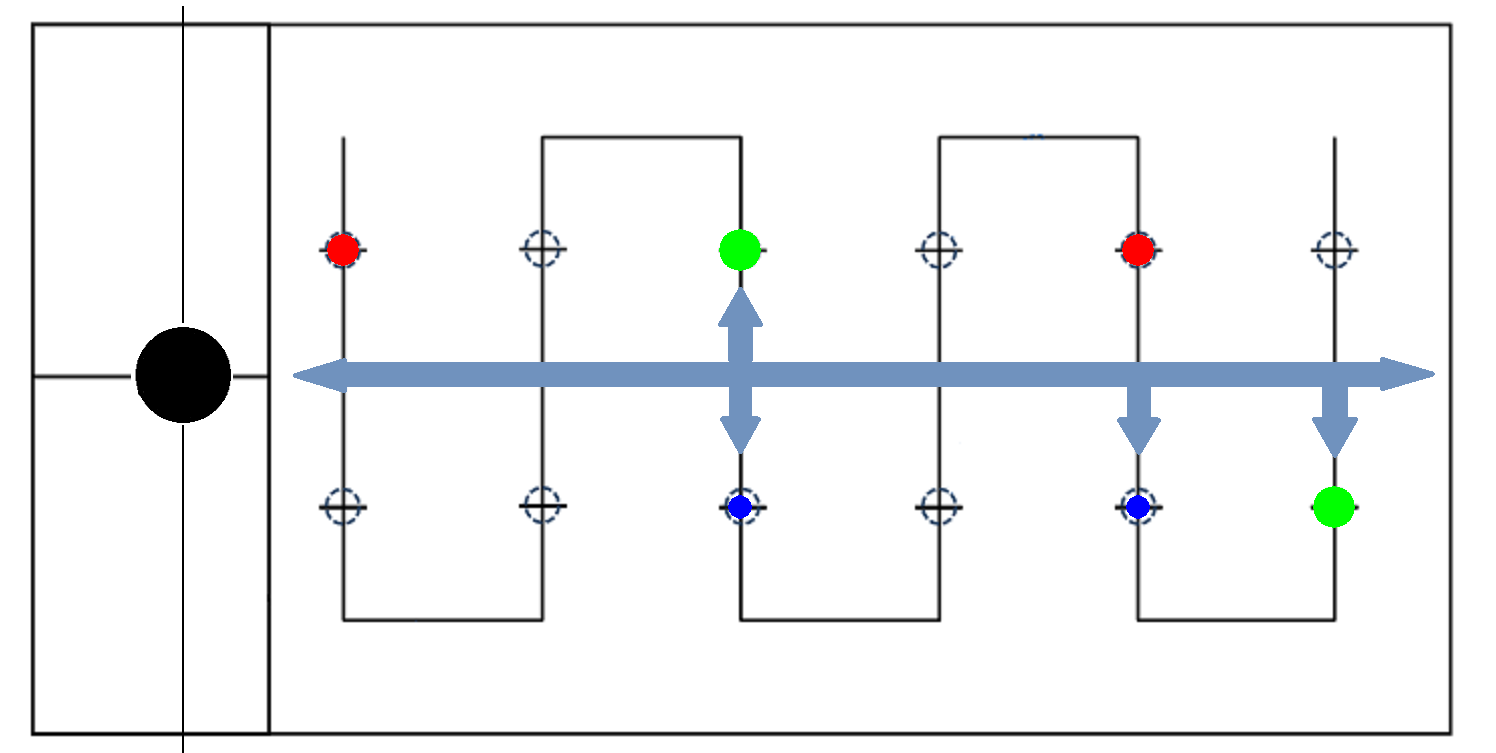
\includegraphics[scale = 0.15]{simu_veh2.png}
        \caption{Phase 2 : transport}
    \end{minipage}
\end{figure}
 
L'accomplissement de la tâche du véhicule se divise en plusieurs phases. La première est une phase de détection durant laquelle le véhicule avance en ligne droite jusqu'au bout du terrain. Il retourne ensuite à son point de départ en ayant en mémoire les emplacements des tubes à prendre et leur diamètres respectifs. La seconde phase se découpe en quatre étapes durant lesquelles le robot va prendre les petits et grands tubes et les ramener dans les zones prévues.
 
De cette simulation, il a pu être démontré que des erreurs de mesures sont présentes dans la réalité et qu'il faut donc construire un programme robuste et précis pour les éliminer. Le principe de ce programme se trouve en annexe dans le code de l'Arduino. De plus, la simulation a permis de vérifier que le temps nécessaire au robot pour réaliser toute la manoeuvre est bien inférieur à 5 minutes, comme indiqué dans le cahier des charges.

\subsection{\label{subsec:simuT}Simulation Turtle}

Elle a pour seul objectif de vérifier la fiabilité de la régulation en position choisie pour contrôler les déplacements du robot. Également programmée dans un environnement \textit{Python}, elle exploite quant à elle le module \textit{Turtle} pour des raison de simplicité par rapport à \textit{PyGame}

\subsubsection{Souci de fidélité du modèle}

Un des objectifs de cette simulation est de se rapprocher de la réalité afin de tirer un maximum des développements simulés.

Le prototype est modélisé par deux roues motrices possédant des caractéristiques physiques similaires aux éléments présentés dans la section \ref{sec:design}: puissance du moteur, diamètre des roues, écarts entre les roues, etc..

Les caractéristiques moteurs sont transposées dans la simulation. En effet, grâce la courbe tension/vitesse (figure \ref{courbe_UV}) linéaire de chacun des deux moteurs (déterminée grâce aux encodeurs optiques), les commandes de tensions des différents moteurs sont transformés en vitesses réelles correspondantes.

\begin{figure}[H]
    \centering
    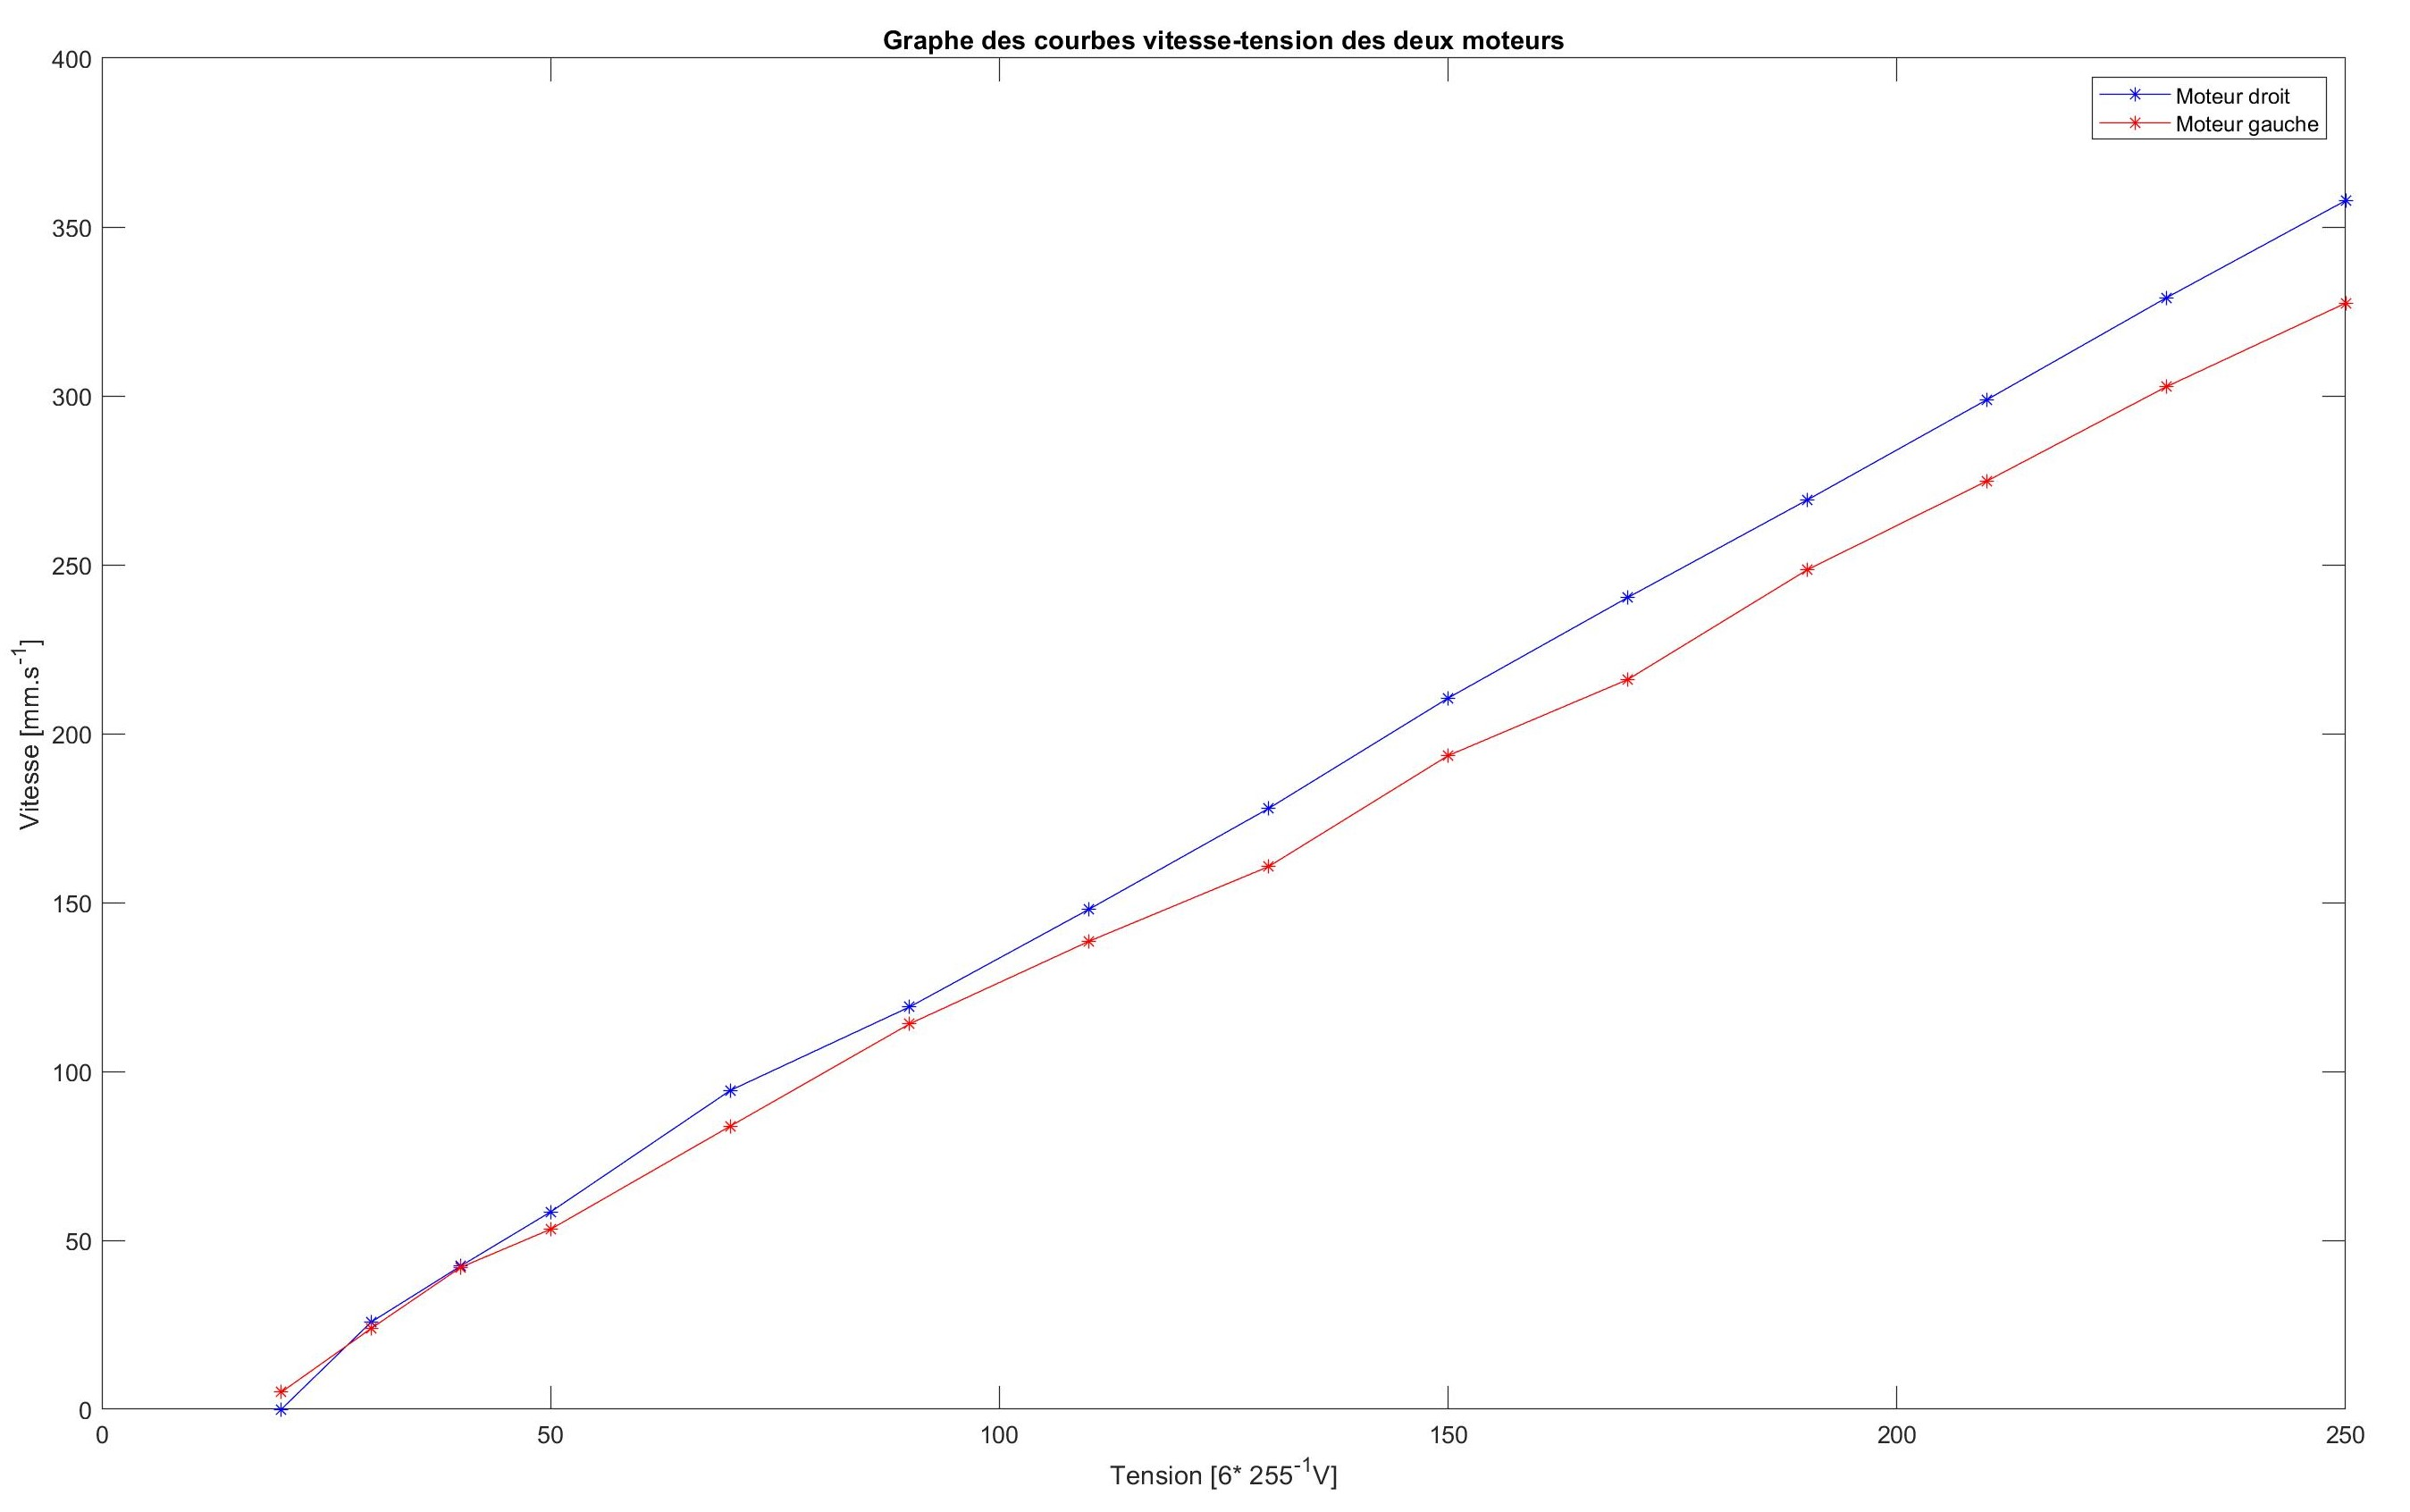
\includegraphics[scale = 0.21]{courbeUV.jpg}
    \captionof{figure}{Graphe des courbes de vitesse-tension des moteurs}
    \label{courbe_UV}
\end{figure}

\subsubsection{Vérification du bon fonctionnement du module de régulation}

La simulation a permis de tester l'efficacité de la plupart des développements mathématiques présents au sein des sections \ref{sec:odo} et \ref{sec:reg}, et ce sans avoir besoin de l'accès au robot. Ceci a été un gain de temps considérable puisqu'il n'a pas fallu attendre la fin de la construction du robot pour avancer sur sa programmation, et que le nombre de tests a pu être grandement augmenté (les tests sont plus rapides sur ordinateur qu'en réalité).

Concernant les modules, seul le bloc odométrie a été remplacé par des fonctions propres de \textit{Turtle}, puisque les encodeurs optiques ne sont pas modélisables. Le bon fonctionnement de tout le reste des modules mathématiques intervenant dans le processus de régulation a été vérifié par la simulation : que ce soit le calcul de la consigne d'angle, de la consigne de distance, de la décomposition de celles-ci en consignes évolutives, de la détermination des profils de vitesses ou du bloc d'asservissement lui-même, en passant par le découpage du déplacement du robot vers un endroit cible en deux séquences, tous ces processus ont été vérifiés avec succès.

Voici des images montrant à quoi peut ressembler la simulation ainsi que l'évolution des différentes variables intervenant dans le régulation à la fin d'exécution d'une consigne. Ici, la consigne donnée en terme de couple (x, y) est (-50,25).
\begin{figure}[H]
    \centering
    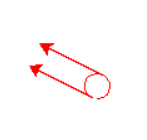
\includegraphics[scale = 1.5]{Capturesimu.PNG}
    \captionof{figure}{Représentation de la trajectoire du prototype lors de l'exécution d'une consigne}
\end{figure}
\begin{figure}[H]
    \centering
    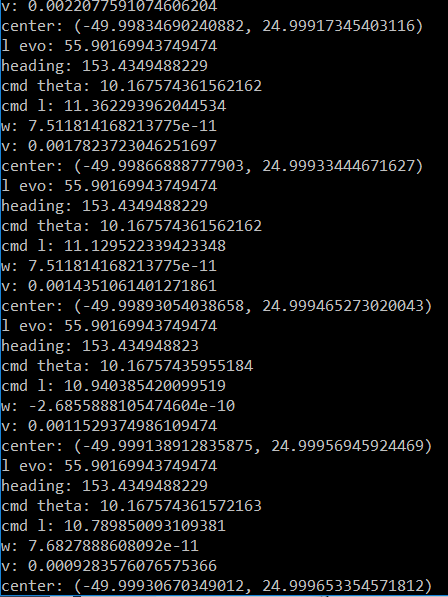
\includegraphics[scale = 1.1]{Capturesimu2.PNG}
    \captionof{figure}{Évolution du centre ainsi que d'autres variables à l'approche de la cible}
\end{figure}

L'entièreté du code de la simulation est disponible en annexe.


\clearpage

\section{\label{sec:4real}Passage à la réalité}

Cette section est consacrée aux problèmes rencontrés par le robot ainsi qu'aux solutions qui ont été apportées pour les résoudre.

\subsection{Système de détection}

Le premier problème survenu durant les phases de tests venait du bruit intervenant dans la détection des tubes, effectuée par les capteurs IR. Pour résoudre cette imprécision causée par des valeurs erronées, il a été décidé de placer, autour de chacun des deux capteurs, un cache permettant de limiter son champ de vision à une zone plus restreinte - se rapprochant de la perpendiculaire partant du capteur. Cette astuce expliquée au point \ref{capteurs} page \pageref{capteurs} a été découverte suite au problème.

Bien que cette modification soit adaptée au problème, certains bruits persistaient rendant la phase de détection inefficace. Une solution plus radicale a donc été ensuite de modifier partiellement la trajectoire du robot durant cette phase. En effet, à la place de détecter les tubes simultanément de part et d'autre du robot en passant au centre de ceux-ci, le prototype suit désormais une trajectoire en forme de "u" afin de passer au plus près des tubes lors de la détection. Ceci n'est plus en total accord avec la stratégie de détection expliquée au point \ref{detec} page \pageref{detec}, puisque l'un des éléments décisifs pour le choix de la détection était la possibilité de trier tous les tubes lors d'un seul passage.

\subsection{Dispositif de préhension}

L'adhérence de la pince a également posé quelques problèmes. Malgré une pression élevée exercée par la pince sur le tube large, ce dernier n'étant pas correctement maintenu et glissait. La solution a été de rajouter du "grip" antidérapant, notamment utilisé sur les manches de raquettes de tennis, pour augmenter suffisamment le frottement de sorte que le tube soit bien maintenu en hauteur. Cette solution est présentée au point \ref{methcstr} page \pageref{methcstr}.

Par ailleurs, lorsque le servomoteur actionnant la fermeture de la pince était soumis à de trop grandes contraintes, la vis de celui-ci tournait folle. Le calibrage effectué sur le servomoteur se déréglait donc à chaque fois. Pour pallier à cette difficulté, la fixation composée d'une vis unique a été repensée pour aboutir à une attache composée de deux vis solidarisant l'ensemble.

\subsection{Design}

Le robot a aussi rencontré un problème d'hyperstaticité du fait qu'il est composé de 4 roues. Les deux ballcasters étant d'abord légèrement plus basses que les deux roues motrices, une de ces deux dernières tournait de temps à autre dans le vide. Pour résoudre ce problème, les ballcasters ont été relevés plus haut que les roues motrices, de sorte que le robot est toujours en isostaticité, changeant de temps à autre de roue libre d'appui.

\subsection{Odométrie}

Comme évoqué à la sous-section \ref{subsec:simuT} page \pageref{subsec:simuT}, le bloc odométrie n'a pu être simulé. C'est pourquoi les tests en temps réel ont cruciaux, d'autant plus que la régulation dépend de l'odométrie. Étonnamment, les résultats obtenus pour le couple de position (x,y) du robot ont été satisfaisants dès les premiers essais, la précision pouvant toutefois être améliorée.

L'orientation du robot déterminant l'état final du robot a posé plus de soucis. Une longue période de débogage à finalement permis de rectifier l'angle renvoyé par l'odométrie, donnant ainsi accès au triplet d'état (x, y, $\theta$) du robot au cours du temps.

En plus de cela, les coefficients de distance jusqu'à lors théoriques (voir section \ref{sec:odo} page \pageref{sec:odo}) ont été remplacés par des coefficients déterminés expérimentalement \cite{guyot_[tutoriel]_2016}. La détermination de ces coefficients de distance gauche et droit consiste à observer les informations relevées par les encodeurs lors de déplacements rectilignes forcés sur une distance connue.

Le module d'odométrie final est donc fonctionnel et précis.

\subsection{\label{subsec:reg4real}Régulation}

Malgré les tests sur simulation, la régulation en temps réel sur le prototype a été très complexe à implémenter. Cependant, le fait d'avoir effectué un déblocage similaire pour la simulation a permis d'obtenir des résultats satisfaisants sous un délais limité.
\clearpage

\section{Résultats et optimisations futures}
Cette section reprend à la fois l'ensemble des résultats obtenus aux termes de ce projet ainsi que les optimisations envisageables dans le futur.

\subsection{Budget}

\begin{figure}[H]
    \centering
    \includegraphics{budget.png}
    \caption{Coût total du robot}
    \label{fig:budget}
\end{figure}

Le robot a bien respecté le cahier des charges en ce qui concerne le budget car le coût total du robot est de 61,33 euros ce qui est largement inférieur au coût maximal de 100 euros. 

\subsection{Design}
En ce qui concerne le produit fini, le prototype est fidèle au design choisi par l'équipe tant au niveau des dimensions que de l'aspect, comme le montrent les figures \ref{fig:robot} et \ref{fig:robot2}. De plus, le robot est à la fois compact, robuste et amovible en ce sens que tous les éléments sont solidaires entre eux tout en restant interchangeables grâce à l'utilisation de \textit{Velcro} en guise de fixation. 
Les optimisations pouvant être faites sont purement esthétiques. Premièrement, l'ensemble des fils électriques pourrait subir une opération de "câble management" afin d'obtenir un aspect visuel plus agréable. Dans la même optique, une sorte de carapace aurait pu être modélisée et fabriquée pour recouvrir l'ensemble du robot en guise de carrosserie cachant les composants électroniques. Par ailleurs, d'un point de vue plus commercial, cela aurait pu représenter la marque de fabrique de notre groupe de recherche et de développement.

\begin{figure}[H]
    \begin{minipage}[c]{.46\linewidth}
        \centering
        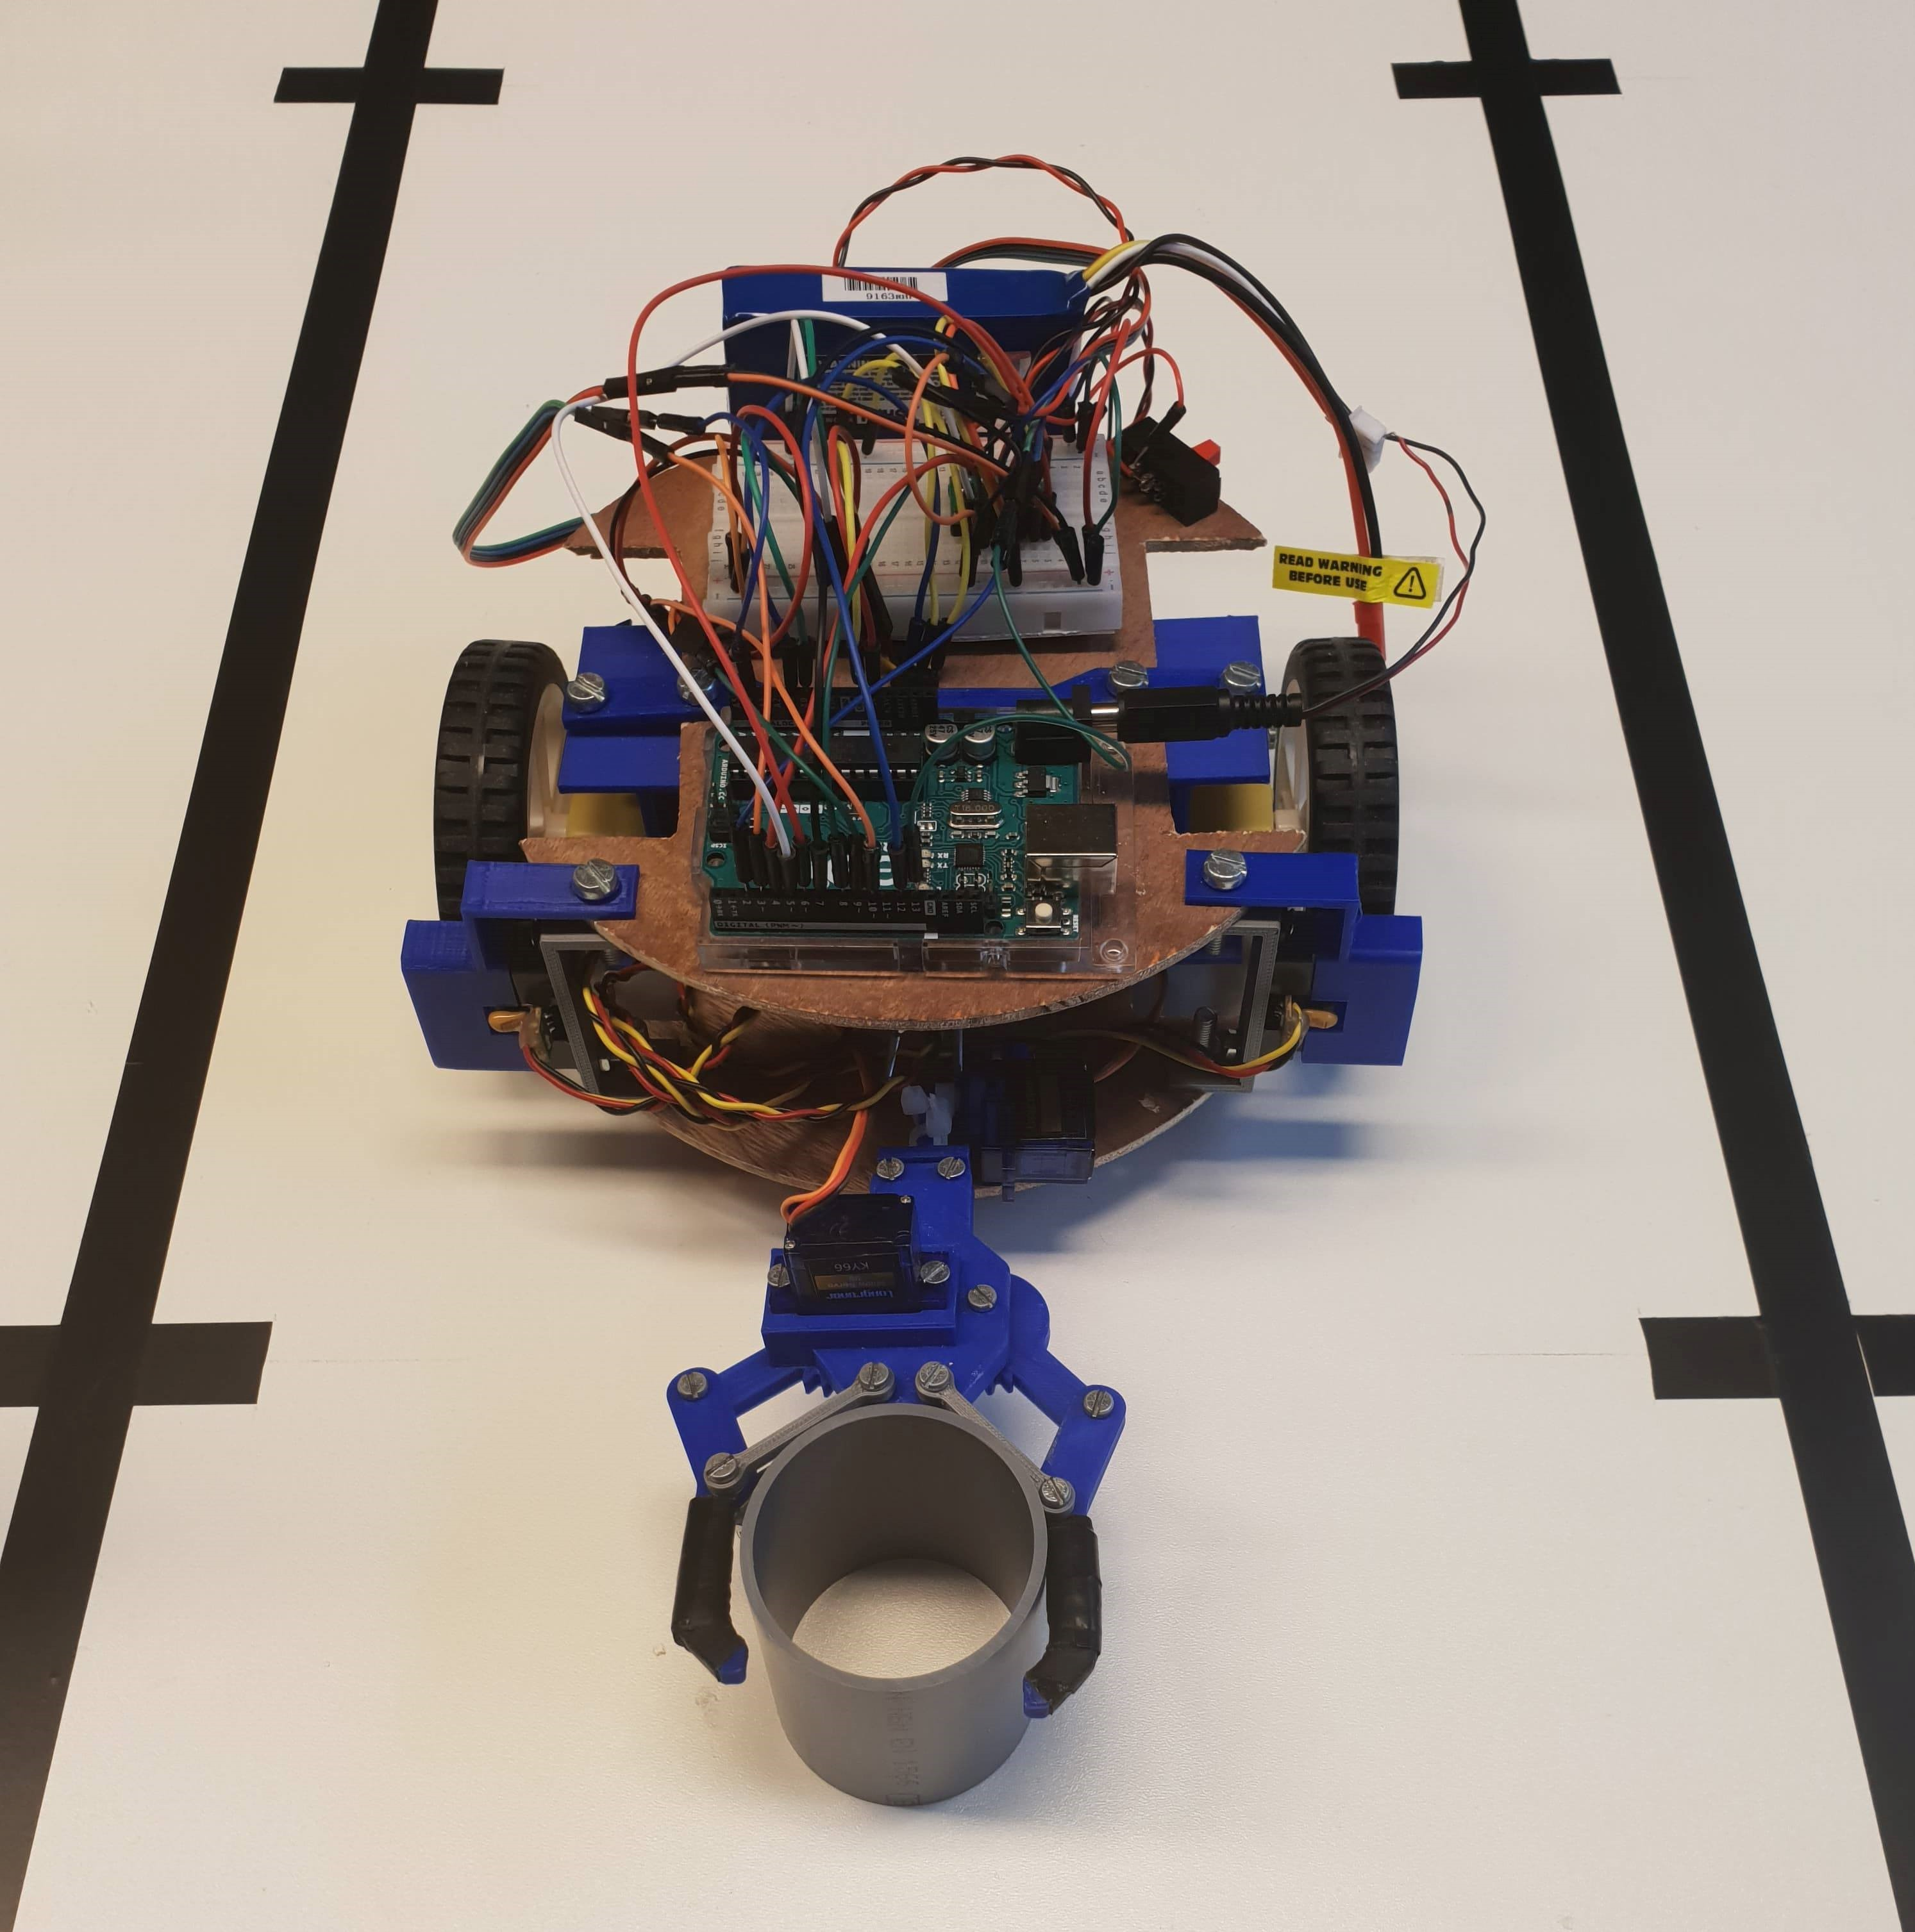
\includegraphics[height = 200]{robot.jpg}
        \captionof{figure}{\label{fig:robot}Prototype vue de face}
    \end{minipage}
    \hfill
    \begin{minipage}[c]{.46\linewidth}
        \centering
        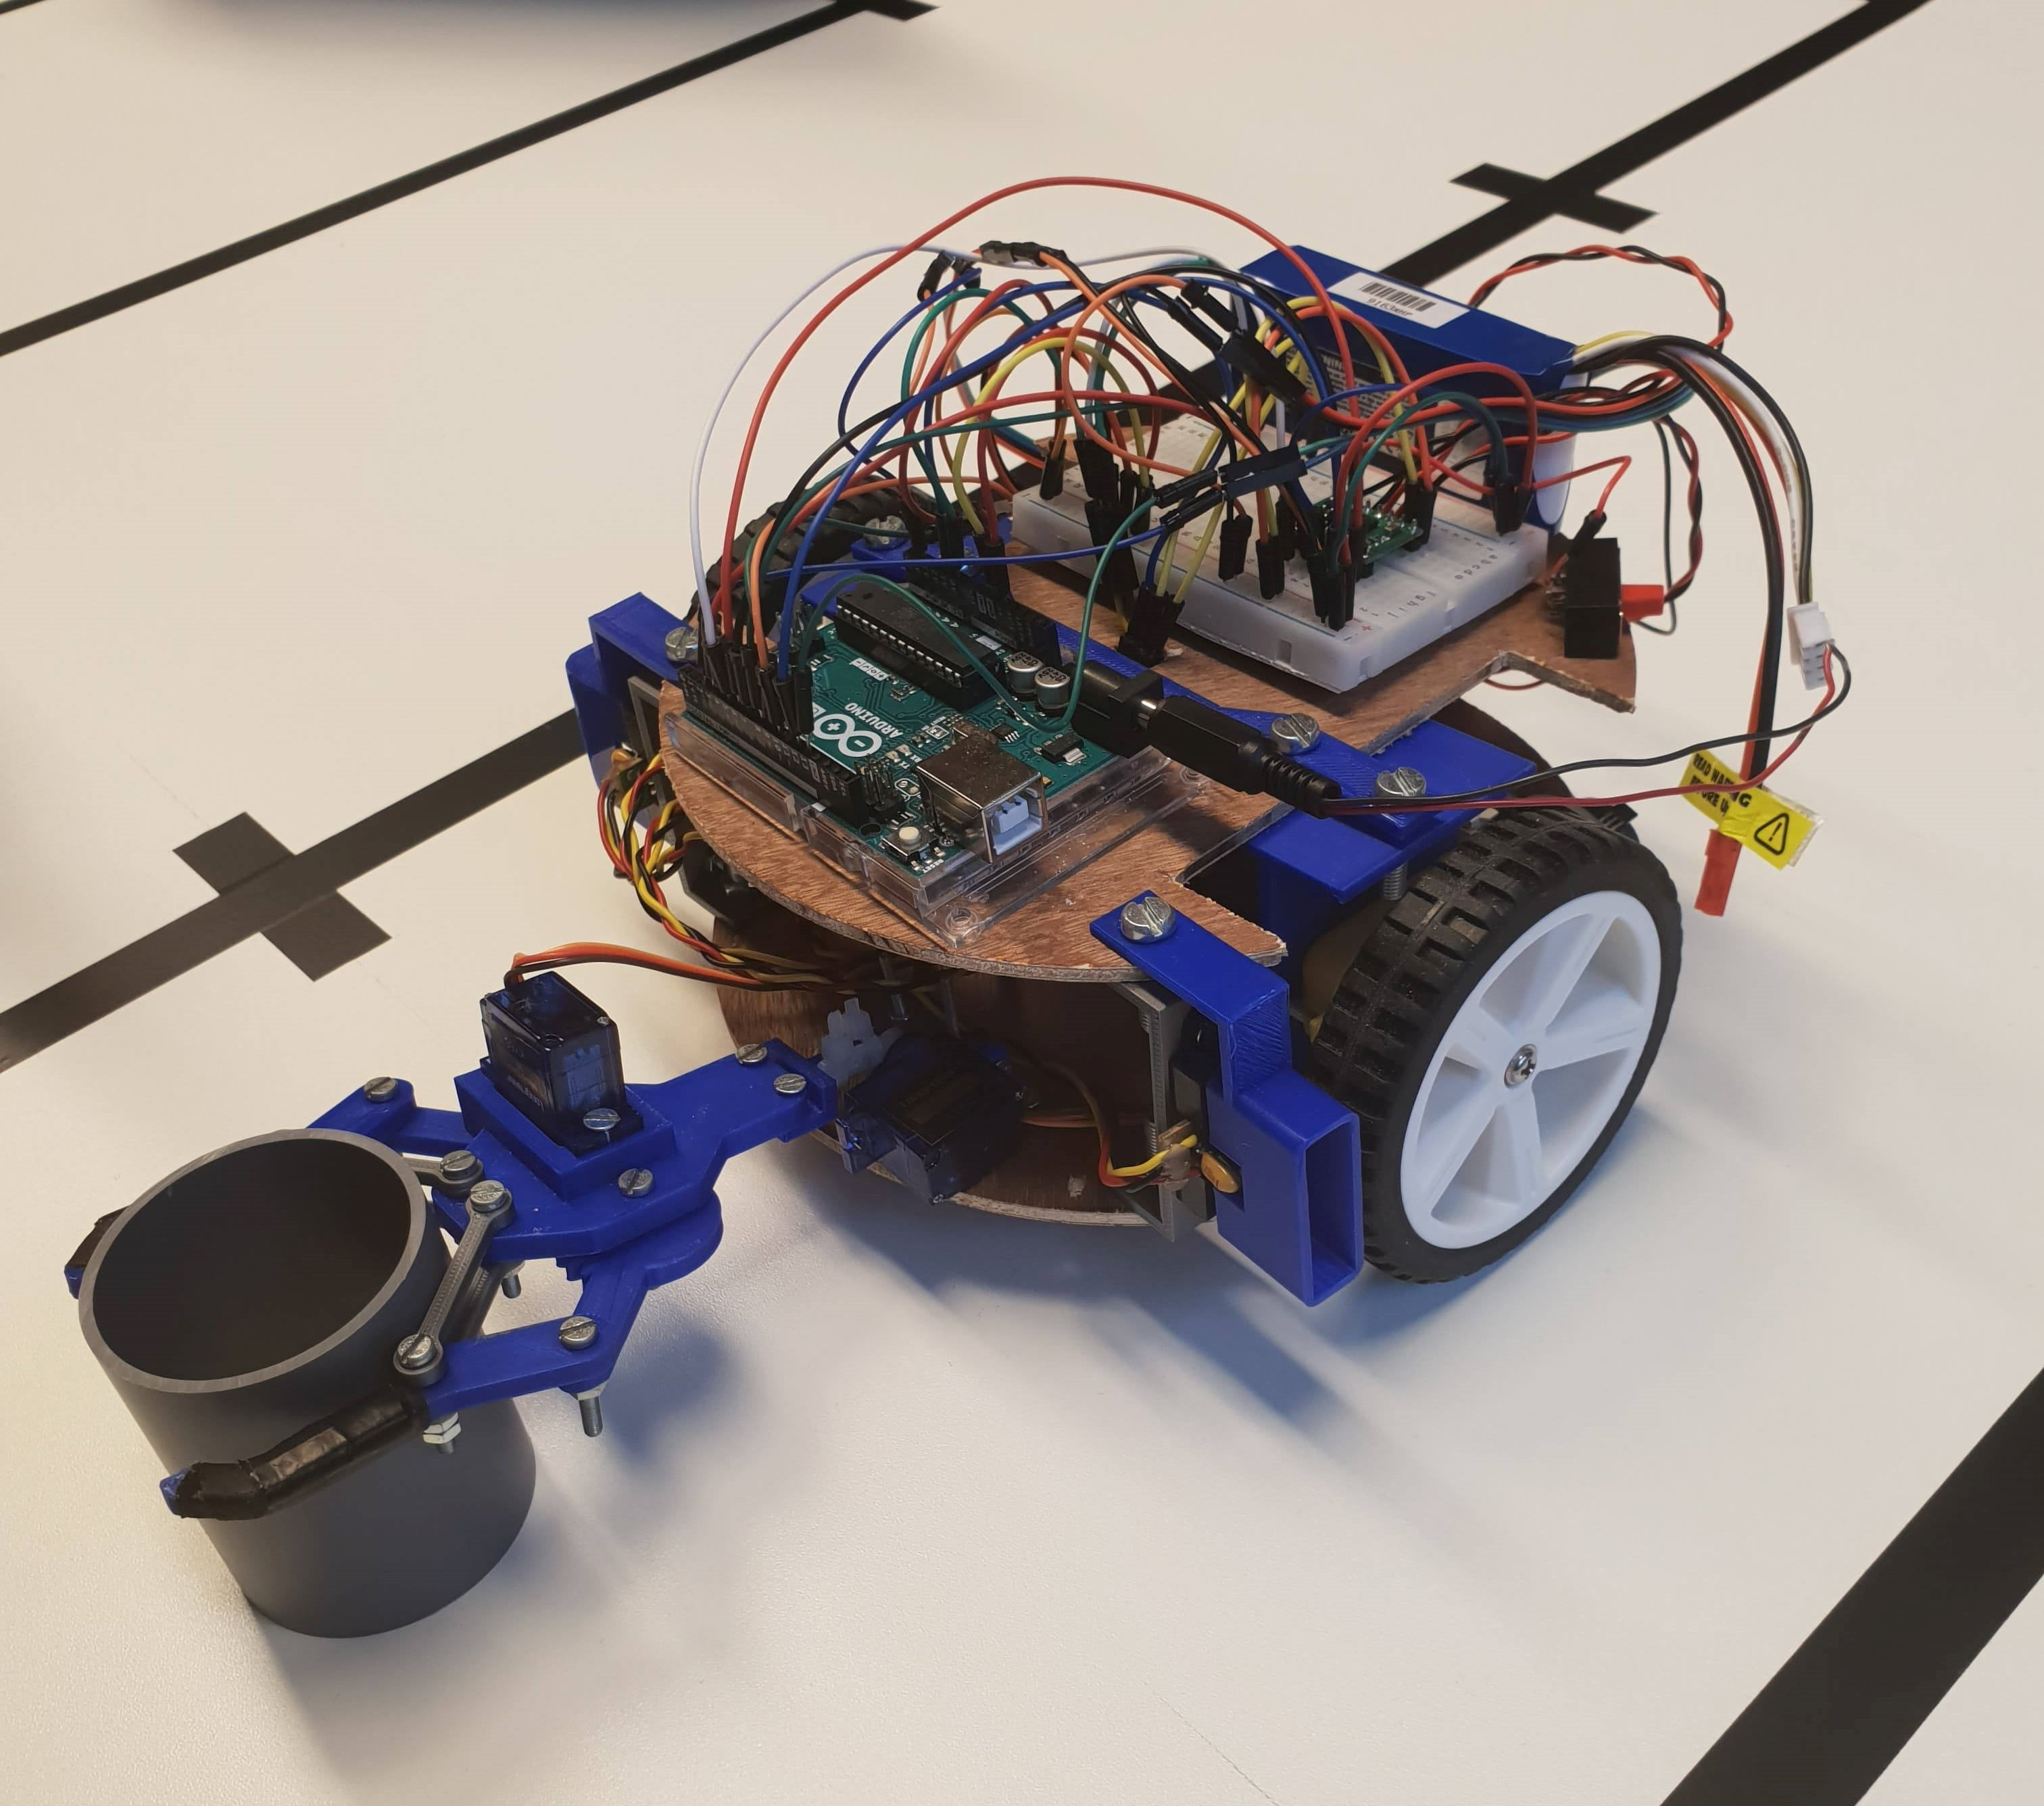
\includegraphics[height = 200]{robot2.jpg}
        \captionof{figure}{\label{fig:robot2}Prototype vue de biais}
    \end{minipage}
\end{figure}

\subsection{Stratégie et fonctionnement}
Au niveau du fonctionnement, chacune des subdivisions de la tâche à réaliser prise séparément sont opérationnelles. En effet, le système de détection permet de distinguer les différents types de tubes par rapport à leur diamètre. La pince saisit et porte les tubes avec succès. La régulation et l'odométrie assurent sans problème le déplacement contrôlé et précis du robot jusqu'au point cible donné tout en respectant les phases de rotation et de mouvement rectiligne. Malgré tout, à l'heure qu'il est, l'enchaînement de ces actions n'est pas encore tout à fait au point - mais cela ne saurait tarder.

Le point fort de notre projet réside dans le fait que le type de robot adopté par l'équipe pour répondre à la mission imposée est des plus communs. En effet, le prototype n'est en aucun cas particularisé à la manoeuvre à effectuer en ce sens qu'il possède les principes de base que requiert un robot intelligent : connaissance de sa position et déplacement contrôlé vers une cible. Seul le programme mettant en place la stratégie d'exécution et le système de préhension est caractéristique du projet, alors que le reste peut être exploité dans la confection de n'importe quel robot autonome. Ainsi, le fonctionnement du robot possède la capacité d'être adapté à une toute autre situation dans un délais minimum.

\subsection{Simulation}

La simulation \textit{Turtle} actuelle a vraiment été d'une grande aide pour comprendre en profondeur comment s'organise une régulation de manière pratique. Elle a permis de relever des problèmes encore non considérés, chacun ayant été progressivement résolu jusqu'à l'obtention de résultats probants. L'intuition obtenue grâce à cette phase de débogage a d'ailleurs grandement facilité l'implémentation de la régulation au robot, comme expliqué à la sous-section \ref{subsec:reg4real} page \pageref{subsec:reg4real}.

En dehors de cela, certains points relatifs à la simulation auraient pu être plus améliorés comme le fait qu'elle soit programmée dans un environnement \textit{Python} (\ref{subsec:simuT} \pageref{subsec:simuT}) et non pas en \textit{langage C} comme doit l'être l'Arduino. Par conséquent, bien que la logique du code soit identique, il a fallu adapter et traduire le programme d'un langage vers l'autre. Travailler la simulation dans un environnement compatible avec le microcontrôleur choisi aurait été un gain de temps. En plus de cela, le souci de fidélité à la réalité évoqué à la section \ref{subsec:simuT} aurait pu être poussé à son paroxysme si des erreurs avaient été insérées au sein du code. Par exemple au niveau des courbes tension/vitesse, pour prendre en compte à la fois les imperfections du terrain et la variation de la puissance envoyée aux moteurs due à la décharge de la batterie. Là où la régulation aurait pu prendre en charge les impuretés de la réalité en plus des consignes, elle ne s'occupe que de ces dernières. Pour finir, une simulation globale aurait été des plus complètes si elle unifiait la simulation sous \textit{PyGame} et celle sous \textit{Turtle}. Cela aurait pu permettre de visualiser la manoeuvre globale et d'en tirer des informations utiles telles que le temps d'exécution.

Si ces différentes améliorations n'ont pas vu le jour, c'est par soucis de facilité et/ou de temps. En effet, il était préférable pour le bien du projet de procéder au plus vite aux essais sur le prototype même étant donné les difficultés éprouvées lors du passage à la réalité.

\clearpage

\section{Project management}

Contrairement au projet de première année, une méthode spécifique (Agile, Scrum, Waterfall, etc.) n'a pas été explicitement suivie, mais l'expérience de chacun avec certaines de celles-ci a permis un déroulement très correct du projet. La méthode résultante a faiblement évolué au cours des semaines, mais s'est toujours adaptée pour une efficacité optimale. De plus, des échéances devaient être respectées. Un rapport bibliographique a du être rédigé pour la fin octobre. Un rapport de mi-parcours a été rendu deux semaines avant le blocus de Noël, et une présentation donnée la semaine suivante pour le premier quadrimestre. L'évaluation finale se déroule la semaine du Printemps des Sciences 2019, tandis que présent rapport (final) et la présentation du robot sont réalisés la semaine précédant le Printemps des Sciences.

\subsection{Réunions}

Pour s'assurer du bon déroulement du projet et de son avancement, notre groupe s'est réuni chaque semaine dans le but de faire un débriefing des dernières avancées et de répartir, le plus équitablement possible, de nouvelles tâches au sein du groupe. Les problèmes rencontrés, préférablement abordés au préalable, y étaient mis sur la table et discutés par l'ensemble. Étaient présents les six membres ainsi que, la plupart du temps, le superviseur.

Lors d'une réunion, un membre jouait le rôle d'animateur pendant qu'un autre, le secrétaire, s'occupait de noter les points principaux. L'animateur préparait l'ordre du jour de la prochaine réunion, au moins la veille de celle-ci. Le secrétaire était chargé d'en rédiger le procès verbal et de le partager au reste du groupe dans les jours qui suivent.

\subsection{Attribution des tâches}

Une bonne façon d'avancer rapidement est d'attribuer, à chaque membre du groupe, une tâche bien précise pour s'assurer qu'elle ait bien été effectuée avant la prochaine réunion. En effet, si le groupe n'a qu'une seule tâche globale à effectuer, tout le monde espérera qu'un autre membre la fasse sans que personne ne s'en occupe.

Si la stratégie première était de faire en sorte que les rôles tournent et que chacun ait l'occasion de toucher à plusieurs aspects du projet, l'apparition de tâches plus longues et les affinités de chacun ont changé la répartition des tâches. Bien que cette façon de faire limitait les nouveaux apprentissages, elle prônait l'exploitation des compétences déjà acquises, ce pour que le travail soit à la fois amoindri quant à sa durée et mieux réalisé. De plus, les nouveaux apprentissages étaient ainsi remplacés par un approfondissement des compétences, et le travail fait par chacun était toujours expliqué et détaillé en réunion.

Ces affinités étaient exploitées pour la construction et l'électronique, pour la régulation et l'odométrie, pour la simulation, pour le code Arduino et le passage de la simulation au code, ou encore pour la rédaction du rapport.

\subsection{Superviseur}

L'ensemble du projet était contrôlé en premier lieu par un superviseur. Son rôle était de veiller au bon déroulement du projet tout en restant passif, c'est-à-dire qu'il ne pouvait pas aider le groupe quant à la réalisation même du prototype - bien qu'il puisse dispenser des conseils et avis. Il assurait également la communication globale entre l'ensemble des superviseurs, les personnes ressources et le groupe.

\subsection{Outils et communication}

\vspace{3mm}
\begin{center}
    \begin{tabular}{l | l}
	Fichiers & Dropbox \\ \hline
	\multirow{2}{*}{Discussion} & Facebook Messenger \\
	           & Slack (partiellement)  \\ \hline
	Rapport & Overleaf \\
\end{tabular}
\vspace{5mm}
\captionof{table}{Récapitulatif des outils employés}
\end{center}

Afin d'améliorer le partage du travail effectué, tous les fichiers ont été mis en ligne sur un dossier Dropbox commun. La discussion générale se déroulait sur Facebook Messenger lorsqu'elle n'était pas possible oralement. Slack a été employé pour la communication spécifique à un aspect du projet (modélisation, code, etc.) au début de celui-ci, mais rapidement abandonné au profit de Messenger. Les rapports de projet étaient rédigés sur un document LaTeX coopératif sur la plateforme Overleaf.
\cleardoublepage

\section{Conclusion}

Pour conclure, ce projet, étalé sur deux quadrimestres, aura débuté par une première phase floue où un cahier des charges (dégagé des consignes) et où la lecture de la littérature (voir rapport bibliographique du premier quadrimestre) en parallèle ont permis l'élaboration d'une stratégie d'exécution de la tâche demandée.

À partir de la stratégie considérée, le design du robot a pu être décidé, tout comme les composants qui le composent désormais, pour finalement le construire et l'adapter tout au long du projet.

Les caractéristiques de ce robot sont l'utilisation poussée d'une odométrie et d'une régulation PI pour son fonctionnement global, l'exploitation d'une détection à distance grâce à des capteurs infrarouges et l'emploi d'une pince pour ramener les tubes un à un dans leur zone propre.

Ces premiers aspects sont décrits synthétiquement dans la première partie du rapport, une partie se voulant axée physique. La deuxième partie du rapport, axée programmation, décrit analytiquement le cheminement ayant mené aux modules essentiels que sont l'odométrie et la régulation, ainsi que l'exploitation de simulations pour parfaire ceux-ci et, préalablement, pour vérifier la stratégie globale.

Le passage à la réalité du programme global et de ses modules a été complexé par divers problèmes, dont l'explication et la résolution sont repris dans le point dédié. 

À l'heure actuelle, le robot effectue toutes les tâches demandées séparément et efficacement. Concernant le comportement pour l'action complète, quelques améliorations sont encore à faire pour que cela fonctionne optimalement, et le robot peut être optimisé plus encore. L'équipe travaille dessus d'arrache-pied afin qu'il soit entièrement fonctionnel pour la présentation finale et le Printemps des Sciences 2019.

Un point analysant la gestion de projet menée durant celui-ci, qui aura été exploitée à bien et aura satisfait tous les membres, clôture le corps du rapport.

Ce projet a été très enrichissant pour chacun, offrant une approche concrète de plus du métier d'ingénieur. Le respect des délais, la prise d'initiative, le travail en équipe prônés seront des aspects fondamentaux durant notre carrière. Les connaissances en robotique, en programmation, en régulation, ou encore en rédaction de rapport ont été élargies pour tous.

% \section{Remerciements}
% Pour le matériel reçu, le code partagé, l'aide quelconque, etc \tdot

\cleardoublepage
\printbibliography[heading=bibintoc, title={Bibliographie}]

\cleardoublepage
\pagenumbering{Alph}
\begin{appendices}

\section{Coordonnées}

\begin{center}
 \begin{tabular}{l | c | r}
    Superviseur & Ir. Max \textsc{Thulliez} & \href{mailto:max.thulliez@ulb.ac.be}{\texttt{max.thulliez@ulb.ac.be}} \\ \hline
    
    Lecteur & Ir. Laurent \textsc{Catoire} & \href{mailto:laurent.catoire@ulb.ac.be}{\texttt{laurent.catoire@ulb.ac.be}} \\ \hline

    \multirow{6}{*}{Auteurs} & Loïc \bsc{Dewitte} & \href{mailto:loic.dewitte@ulb.ac.be}{\texttt{loic.dewitte@ulb.ac.be}} \\
            & Maxime \bsc{Renard} & \href{mailto:maxime.renard@ulb.ac.be}{\texttt{maxime.renard@ulb.ac.be}} \\
            & Théo \bsc{Saclier} & \href{mailto:theo.saclier@ulb.ac.be}{\texttt{theo.saclier@ulb.ac.be}} \\
            & Firas \bsc{Samaan} & \href{mailto:firas.samaan@ulb.ac.be}{\texttt{firas.samaan@ulb.ac.be}} \\
            & Tristan \bsc{Smeesters} & \href{mailto:tristan.smeesters@ulb.ac.be}{\texttt{tristan.smeesters@ulb.ac.be}} \\
            & Julien \bsc{van Delft} & \href{mailto:julien.van.delft@ulb.ac.be}{\texttt{julien.van.delft@ulb.ac.be}} \\
\end{tabular}   
\end{center}

\section{Codes}

\begin{figure}[H]
    \centering
    \includegraphics[scale = 0.75]{code1.png}
 \end{figure}

\begin{figure}[H]
    \centering
    \includegraphics[scale = 0.75]{code2.png}
\end{figure}
 
\begin{figure}[H]
    \centering
    \includegraphics[scale = 0.75]{code3.png}
\end{figure}

\begin{figure}[H]
    \centering
    \includegraphics[scale = 0.75]{code4.png}
\end{figure}

\begin{figure}[H]
    \centering
    \includegraphics[scale = 0.75]{code5.png}
\end{figure}

\begin{figure}[H]
    \centering
    \includegraphics[scale = 0.75]{code6.png}
\end{figure}

\begin{figure}[H]
    \centering
    \includegraphics[scale = 0.75]{code7.png}
\end{figure}

\begin{figure}[H]
    \centering
    \includegraphics[scale = 0.7]{code8.png}
\end{figure}

\begin{figure}[H]
    \centering
    \includegraphics[scale = 0.75]{code9.png}
\end{figure}

\begin{figure}[H]
    \centering
    \includegraphics[scale = 0.75]{code10.png}
\end{figure}

\begin{figure}[H]
    \centering
    \includegraphics[scale = 0.75]{code11.png}
\end{figure}

\begin{figure}[H]
    \centering
    \includegraphics[scale = 0.75]{code12.png}
\end{figure}

\begin{figure}[H]
    \centering
    \includegraphics[scale = 0.75]{code13.png}
\end{figure}

\begin{figure}[H]
    \centering
    \includegraphics[scale = 0.75]{code14.png}
\end{figure}

\begin{figure}[H]
    \centering
    \includegraphics[scale = 0.75]{code15.png}
\end{figure}

\begin{figure}[H]
    \centering
    \includegraphics[scale = 0.75]{code16.png}
\end{figure}

\begin{figure}[H]
    \centering
    \includegraphics[scale = 0.75]{code17.png}
\end{figure}
\end{appendices}

\usepackage[final]{pdfpages}
\includepdf[pages=-]{code.pdf}


\end{document}